\documentclass[10pt, letterpaper]{report}
% !TeX program = xelatex
%==================PREAMBOLO=======================%
\usepackage[utf8]{inputenc}
\usepackage{psvectorian}
\usepackage{pgfplots}
\usepackage[Rejne]{fncychap}
\usepackage[export]{adjustbox}
\usepackage[T1]{fontenc}
\usepackage{lmodern}
\usepackage[shortlabels]{enumitem}
\usepackage{moresize}
\usepackage{graphicx} % Required for inserting images
\usepackage{hyperref}
\usepackage{listings}
\usepackage[table,xcdraw]{xcolor}
\usepackage{amssymb}
\usepackage{amsmath}
\usepackage[italian]{babel}
\usepackage{nicefrac, xfrac}
\usepackage{tikz}
\usepackage{mathrsfs} 
\usepackage{titletoc}
\usepackage{fancyhdr}
\usepackage{psvectorian,lipsum}
\usepackage{fourier-orns}
\usepackage{lipsum}
\usepackage[paper=a4paper,left=25mm,right=25mm,bottom=25mm,top=25mm]{geometry}
\definecolor{light-gray}{gray}{0.95}
\definecolor{cop}{HTML}{f7ecd7}
\definecolor{copAut}{HTML}{ababab}
\definecolor{copAut2}{HTML}{c3c3e6}
\definecolor{purcop}{HTML}{d0d3db}
\definecolor{sapienza}{HTML}{660f1d}
\definecolor{lightSapienza}{HTML}{e3d3d5}
\definecolor{darkgreen}{HTML}{008000}
\definecolor{cartaRiciclata}{HTML}{fcfcf7}
\newcommand{\redText}[1]{\color{red}#1\color{black}}
\newcommand{\code}[1]{\colorbox{light-gray}{\texttt{#1}}}
\newcommand{\codee}[1]{\colorbox{white}{\texttt{#1}}}
\newcommand{\K}{{\mathbb K}}
\newcommand{\notimplies}{%
  \mathrel{{\ooalign{\hidewidth$\not\phantom{=}$\hidewidth\cr$\implies$}}}}
\newcommand{\flowerLine}{ \begin{center}\decofourleft\hphantom{ }\decoone\hphantom{ }\decofourright\hphantom{}\hphantom{aa}
\decofourleft\hphantom{ }\decoone\hphantom{ }\decofourright\hphantom{}\hphantom{aa}
\decofourleft\hphantom{ }\decoone\hphantom{ }\decofourright\hphantom{}\hphantom{aa}
\decofourleft\hphantom{ }\decoone\hphantom{ }\decofourright\hphantom{}\hphantom{aa} 
\decofourleft\hphantom{ }\decoone\hphantom{ }\decofourright\hphantom{}\hphantom{aa}
\decofourleft\hphantom{ }\decoone\hphantom{ }\decofourright\hphantom{}\hphantom{aa}
\decofourleft\hphantom{ }\decoone\hphantom{ }\decofourright\hphantom{}\hphantom{aa}
\decofourleft\hphantom{ }\decoone\hphantom{ }\decofourright\hphantom{}\hphantom{aa}
\decofourleft\hphantom{ }\decoone\hphantom{ }\decofourright\hphantom{}\hphantom{aa}
\end{center}}
\definecolor{g}{RGB}{60, 50, 50}
\newcommand{\textg}[1]{\color{g}{\textbf{#1}}\color{black}}
\newcommand{\teo}[1]{{\large\color{sapienza}\textbf{Teorema #1 :\hphantom{a}}}}
\newcommand{\defi}[1]{{\large\color{sapienza}\textbf{Definizione #1 :\hphantom{a}}}}
\newcommand{\claim}[1]{{\color{sapienza}\textbf{Claim #1 :\hphantom{a}}}}
\newcommand{\lemma}[1]{{\color{sapienza}\textbf{Lemma #1 :\hphantom{a}}}}
\newcommand{\dimo}[1]{{\color{sapienza}\textbf{Dimostrazione #1 :\hphantom{a}}}}
\newcommand{\prop}[1]{{\color{sapienza}\textbf{Proposizione #1 :\hphantom{a}}}}
\newcommand\greybox[1]{%
  \vskip\baselineskip%
  \par\noindent\colorbox{light-gray}{%
    \begin{minipage}{\textwidth}#1\end{minipage}%
  }%
  \vskip\baselineskip%
}
\newcommand\sapbox[1]{%
  \vskip\baselineskip%
  \par\noindent\colorbox{lightSapienza}{%
    \begin{minipage}{\textwidth}#1\end{minipage}%
  }%
  \vskip\baselineskip%
}

\newcommand{\Z}{{\mathbb Z}}
\newcommand{\blank}{{\sqcup}}
\newcommand{\R}{{\mathbb R}}
\newcommand{\N}{{\mathbb N}}
\newcommand{\C}{{\mathbb C}}
\newcommand{\Sn}{{\mathcal S_n}}
\newcommand{\An}{{\mathcal A_n}}
\newcommand{\E}{{\mathcal E}}
\newcommand{\B}{{\mathcal B}}
\newcommand{\mcm}{{\text{mcm}}}
\newcommand{\rg}{{\text{rg}}}
\newcommand{\ve}{{\bar v}}
\newcommand{\spaz}{{\text{\hphantom{aa}}}}
\newcommand{\MCD}{{\text{MCD}}}
\newcommand{\tc}{{\text{ tale che }}}
\newcommand{\supp}{{\text{Supp}}}
\newcommand{\acc}{\\\hphantom{}\\}
\newcommand{\aut}{{\text{Aut}}}
\newcommand{\Span}{{\text{Span}}}
\newcommand{\End}{{\text{End}}}
\newcommand{\cen}{{\text{Centro}}}
\newcommand{\norm}{{\unlhd}}
\newcommand{\ciclS}{{\left \langle }}
\newcommand{\ciclE}{{\right \rangle }}
\newcommand{\boxedMath}[1]{\begin{tabular}{|c|}\hline \texttt{#1} \\ \hline\end{tabular} :}
\newcommand{\shell}[1]{\colorbox{black}{\textcolor{white}{\texttt{#1}}}}
\newcommand{\eqImportante}[1]{\begin{center}\huge\lefthand\hphantom{a}
    \normalsize\texttt{#1}
    \hphantom{aaa}\huge\righthand\end{center}}

\fancyhf{}
\pagestyle{fancy}
\usepackage{pgf-pie}  
\usetikzlibrary{positioning}

\renewcommand{\headrule}{%
\vspace{-8pt}\hrulefill
\raisebox{-2.1pt}{\quad\decothreeleft\decotwo\decothreeright\quad}\hrulefill}

%sta roba serve per il codice C
\definecolor{mGreen}{rgb}{0,0.6,0}
\definecolor{mGray}{rgb}{0.5,0.5,0.5}
\definecolor{mPurple}{rgb}{0.58,0,0.82}
\definecolor{backgroundColour}{rgb}{0.95,0.95,0.92}

\lstdefinestyle{CStyle}{
    backgroundcolor=\color{backgroundColour},   
    commentstyle=\color{mGreen},
    keywordstyle=\color{magenta},
    numberstyle=\tiny\color{mGray},
    stringstyle=\color{mPurple},
    basicstyle=\footnotesize,
    breakatwhitespace=false,         
    breaklines=true,                 
    captionpos=b,                    
    keepspaces=true,                 
    numbers=left,                    
    numbersep=5pt,                  
    showspaces=false,                
    showstringspaces=false,
    showtabs=false,                  
    tabsize=2,
    language=C
}
\lstdefinestyle{CppStyle}{
    backgroundcolor=\color{backgroundColour},   
    commentstyle=\color{mGreen}\ttfamily,
    morecomment=[l][\color{magenta}]{\#}
    keywordstyle=\color{blue}\ttfamily,
    numberstyle=\tiny\color{mGray},
    stringstyle=\color{red}\ttfamily,
    basicstyle=\ttfamily,
    breakatwhitespace=false,         
    breaklines=true,                 
    captionpos=b,                    
    keepspaces=true,                 
    numbers=left,                    
    numbersep=5pt,                  
    showspaces=false,                
    showstringspaces=false,
    showtabs=false,                  
    tabsize=2,
    language=C
}
\lstset{language=C++,
                basicstyle=\ttfamily,
                keywordstyle=\color{blue}\ttfamily,
                stringstyle=\color{red}\ttfamily,
                commentstyle=\color{green}\ttfamily,
                morecomment=[l][\color{magenta}]{\#}
}
%fine roba che serve per il codice C
\usepackage{minted}
 %TOGLI COMMENTO SE USI XELATEX
%\usepackage{fontspec}
\title{\jobname} %========TITOLO========%
\author{Marco Casu}
\date{\vspace{-5ex}}
\begin{document}

%==================COPERTINA=======================%
\begin{titlepage}
    \pagecolor{cartaRiciclata}
\begin{center}
    %TOGLI COMMENTO SE USI XELATEX
   %\setmainfont{Palace Script MT}
   \HUGE Marco Casu\acc
    %\setmainfont{Grand Casino}
     %TOGLI COMMENTO SE USI XELATEX
    %\setmainfont{h Halfroad}
    \HUGE \decothreeleft\hphantom{ }{\fontsize{48}{50}\selectfont \jobname}\hphantom{ }\decothreeright
     %TOGLI COMMENTO SE USI XELATEX
   % \setmainfont{Times New Roman}
\end{center}
\thispagestyle{empty}
\begin{figure}[h]
    \centering{
        %l'immagine deve avere una risoluzione 2048x2048
        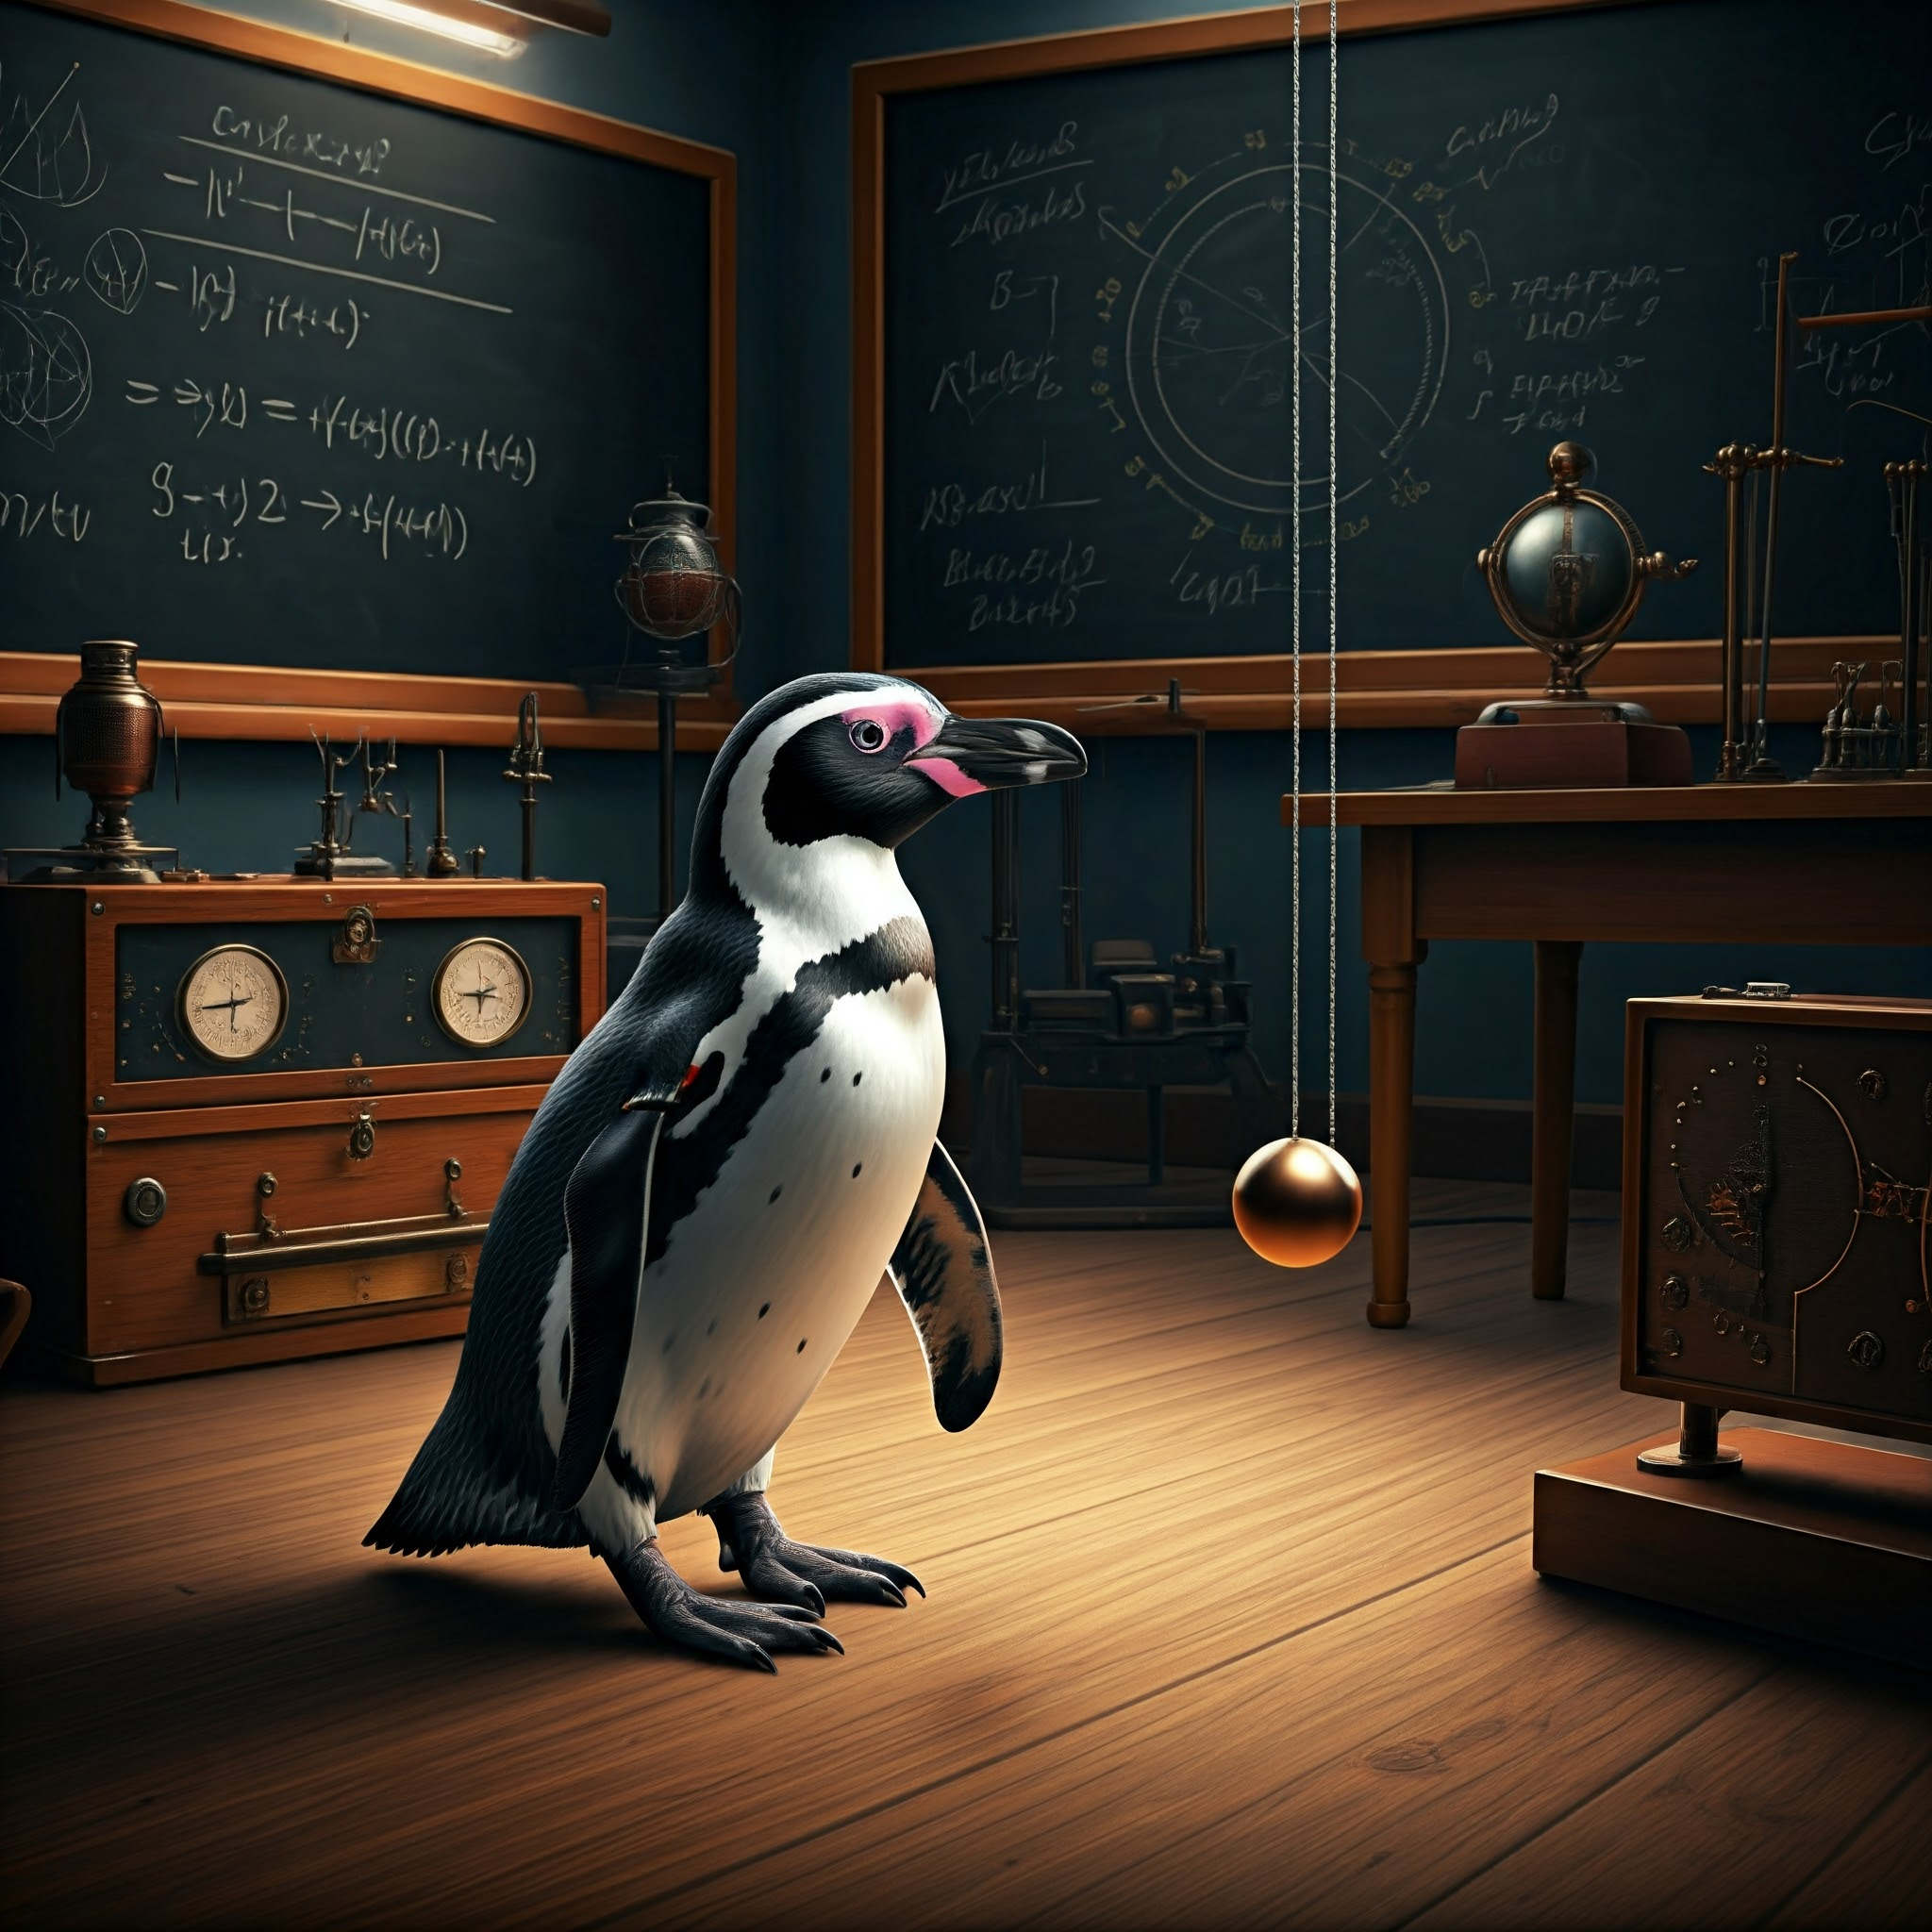
\includegraphics[width=1\textwidth ]{images/copertina.jpg}
    }
\end{figure}
\vfill 
\centering 
\includegraphics[width=0.4\textwidth ]{../../preamble/Stemma_sapienza.png} \acc
\centering \Large \color{sapienza}Facoltà di Ingegneria dell'Informazione,
Informatica e Statistica\\
Dipartimento di Informatica
\end{titlepage}

%===================FINE COPERTINA======================%
\newpage
\pagecolor{cartaRiciclata}%\setmainfont{Algerian}
Questo documento è distribuito sotto la licenza 
\color{blue}\href{https://www.gnu.org/licenses/fdl-1.3.txt}{GNU}\color{black},  
è un resoconto degli appunti (eventualmente integrati con libri di testo) tratti dalle lezioni del corso di \jobname
\hphantom{a}per la laurea 
triennale in Informatica. Se dovessi notare errori, ti prego di segnalarmeli.
\vfill
\begin{figure}[h!]
    \raggedright
    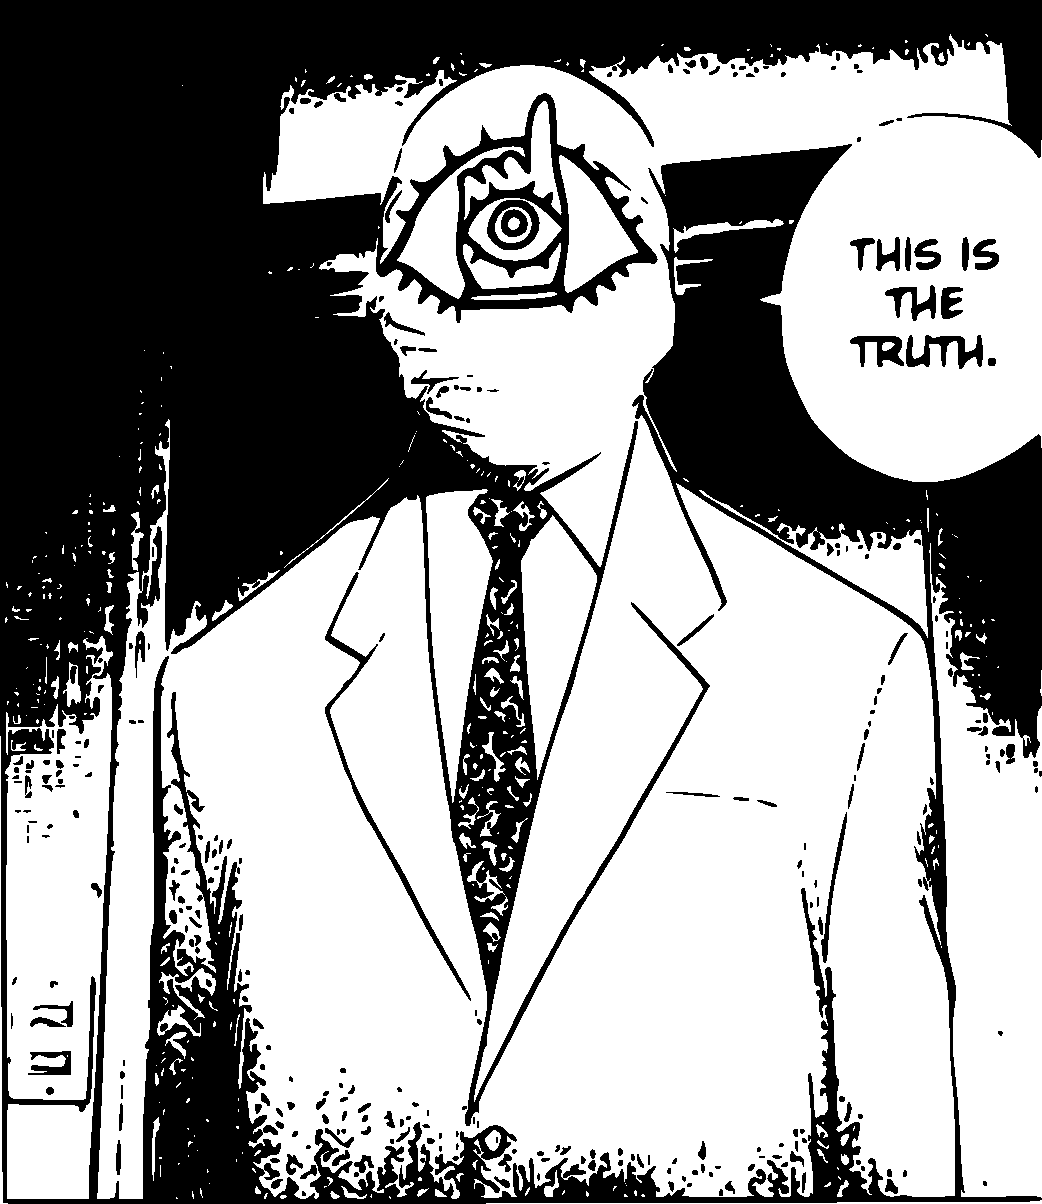
\includegraphics[width=0.4\textwidth,right ]{../../preamble/tomodachi.pdf} 
\end{figure}
\newpage %\setmainfont{Times New Roman}
\normalsize
\tableofcontents 
\newpage

%==================FOOTER e HEADER=======================%
\fancyhf{}
\fancyhead[L]{\nouppercase{\leftmark}}
\fancyhead[R]{Sezione \thesection}
\fancyfoot[C]{\thepage}
\fancyfoot[L]{Appunti di \jobname}
\fancyfoot[R]{ Marco Casu}
%\fancyfoot[R]{\setmainfont{Palace Script MT}\huge Marco Casu \setmainfont{Times New Roman}}
%==================FOOTER e HEADER=======================%

%Ricorda del comando \flowerLine per separare le sottosezioni. Le sezioni si separano nelle diverse pagine

%==================INIZIO======================%

\chapter{Introduzione}
\section{Il metodo scientifico}
La nascita del metodo scientifico è dovuta a Galileo Galilei, se i filosofi greci stabilivano 
leggi empiriche senza necessariamente dimostrarle, Galileo introdusse una verifica sperimentale 
a quelle che erano le sue digressioni.\acc 
Un \textbf{esperimento}, è una verifica sperimentale delle ipotesi, utile a ricavare valori 
numerici oggettivi per le misure delle grandezze fisiche. L'avvento del cannocchiale permise un 
osservazione più accurata dei corpi celesti, questi che venivano creduti perfetti, si rivelarono 
per quello che sono, la Luna con i suoi accavallamenti e "mari", mostrava una 
conformazione della sua crosta tutto fuorché perfetta.
\begin{figure}[h!]
    \centering
    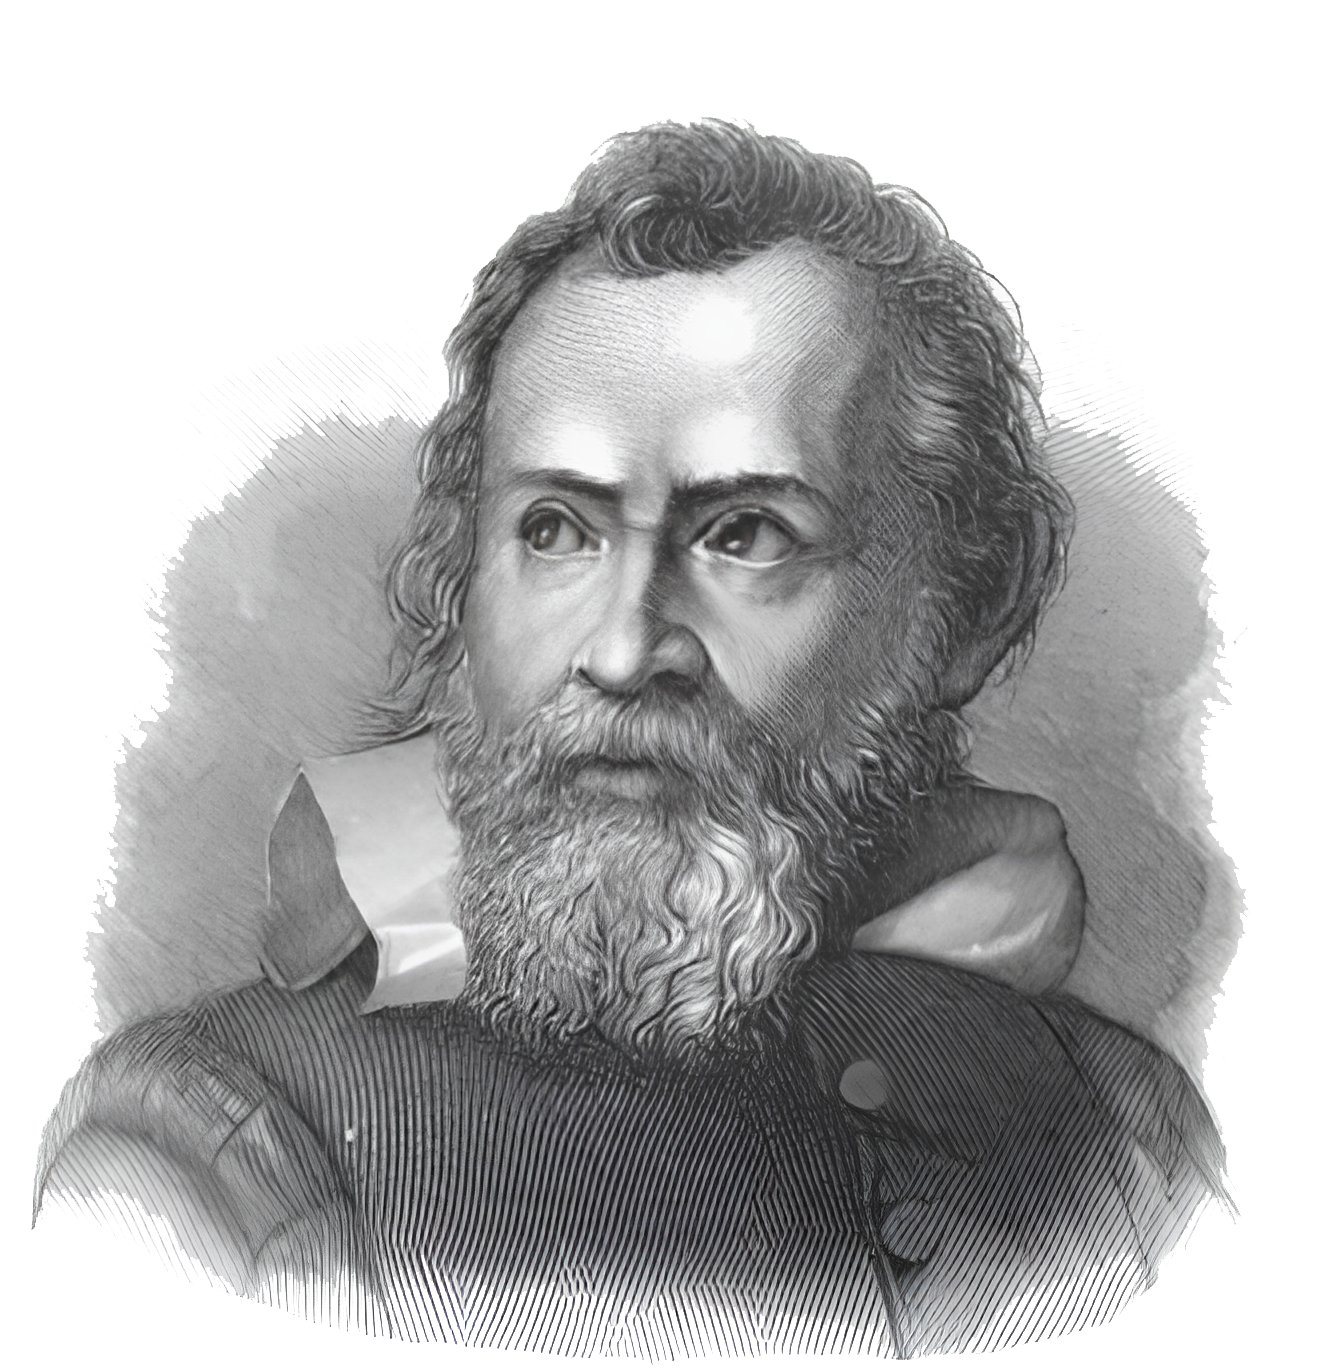
\includegraphics[width=140pt]{images/Galileo2.png}
    \caption{ Galileo Galilei}
    \label{fig:Galileo}
\end{figure}
Oltre al già citato cannocchiale, erano necessari ulteriori strumenti per le osservazioni dei 
corpi celesti, era necessario misurare in maniera precisa ed affidabile lo scorrere del tempo. 
Misurare il tempo vuol dire confrontare due eventi, ad esempio, il sorgere del sole con il movimento 
periodico riferito ad un misuratore (come l'orologio).\acc 
Galileo per le sue misure realizzò un orologio ad acqua, utilizzando un recipiente nella quale 
riporre un piccolo foro sul fondo, in modo tale che l'acqua cadesse a gocce a velocità costante, 
così facendo, lo scorrere del tempo era proporzionale al volume dell'acqua perso dall recipiente.\acc 
Una \textbf{grandezza fisica} è un entità alla quale si attribuisce una specifica definizione, utilizzabile 
per descrivere un fenomeno fisico, per tali entità devono valere i criteri di uguaglianza e 
sommabilità.\acc 
Uno degli argomenti su cui si soffermò Galileo fu il \textit{moto dei gravi}, in particolare 
il moto dei corpi in caduta libera. Secondo la fisica aristotelica del tempo, un corpo 
tanto più pesante era, tanto più rapidamente cadeva. \acc 
Galileo fu critico nei riguardi di questa visione, osservò che in realtà, ogni corpo 
cade verso il suolo con la stessa accelerazione, il motivo per il quale una piuma cade 
più rapidamente di una sfera di piombo non riguarda la loro massa, bensì la resistenza dell'aria 
nei confronti del loro materiale e della loro forma. Trovò inoltre che la distanza percorsa 
durante la caduta di un oggetto è proporzionale al quadrato del tempo impiegato per percorrerla.\acc 
Galileo con un esperimento riguardante i piani osservò il seguente fatto : 
    \textit{se si lascia scivolare un corpo su un piano inclinato ad altezza $h$ per poi 
    farlo risalire su un altro piano inclinato, questo tendeva a risalire fino alla 
    stessa altezza $h$}.
    \begin{figure}[h!]
        \centering
        \includegraphics[width=500pt]{images/cadutaGraveBW.eps}
        \caption{ caduta sul piano inclinato}
        \label{fig:caduta}
    \end{figure}\acc
Inoltre, notò che questo fenomeno non è condizionato dal seno dell'angolo del piano, bensì 
esclusivamente dall'altezza.
\begin{figure}[h!]
    \centering
    \includegraphics[width=500pt]{images/cadutaGrave2BW.eps}
    \caption{ inclinazioni differenti}
    \label{fig:caduta2}
\end{figure}\acc
Per osservare tale risultato dovette ridurre le azioni spurie dell'attrito dell'aria. Più 
il percorso era liscio, più l'attrito risultava debole, e più il corpo tendeva ad 
avvicinarsi all'altezza originale $h$. Con tale ragionamento ipotizzò che se l'attrito dovesse 
essere stato nullo, allora il corpo sarebbe tornato precisamente all'altezza $h$.\acc 
Dato questo per vero, riducendo il valore dell'angolo sarebbe stato possibile far percorrere 
al corpo una distanza maggiore. Se il secondo piano avesse avuto inclinazione nulla, allora 
il grave avrebbe continuato a muoversi in avanti a velocità costante.\begin{figure}[h!]
    \centering
    \includegraphics[width=330pt]{images/cadutaGrave3BW.eps}
    \caption{ inclinazione nulla}
    \label{fig:caduta3}
\end{figure}\acc
Tale principio è noto come \textbf{legge d'Inerzia}, eliminando gli attriti, lo stato di moto naturale inalterato di
un corpo è quello di moto rettilineo uniforme (a velocità costante) indefinitamente.\acc 
Essendo la scienza sempre stata impiegata anche in ambito bellico, Galileo studiò il moto dei 
proiettili, che fino a quel momento si credeva fosse costantemente orizzontale, fino al momento in 
cui il proiettile perdeva il suo "impeto" cadendo a terra. Egli si rese conto che 
i proiettili sono soggetti sia alla forza impressa dal colpo (orizzontale), sia a quella verticale 
impressa verso il basso.\acc 
La forza impressa dal colpo gli da una velocità costante, in quanto non è soggetto ad ulteriori 
accelerazioni orizzontalmente, quella verticale invece provoca un moto uniformemente accelerato, 
la distanza 
percorsa in verticale è proporzionale al 
quadrato del tempo impiegato a percorrerla, la combinazione dei due moti risulta in un arco 
di parabola.
\begin{center}
	\begin{tabular}{>{\centering\arraybackslash}m{3in}>{\centering\arraybackslash}m{3in}}
		\begin{tikzpicture}[scale=0.9, transform shape]
		\begin{axis}[
		ymin=-6,
		ymax = 6,
		xmin=-6,
		xmax = 6,
		axis lines = center,
		xtick distance=2, ytick distance=2,
		grid style=dashed,
		ymajorgrids=true,
		xmajorgrids=true,
		xlabel = \(\),
		ylabel = {\(\)},
		]
		%Below the red parabola is defined
		\addplot [
		domain=-6:6,
		samples=20,
		color=blue,
		]
		{-(1/5)*(x^2)};
		\addlegendentry{\(y=-\nicefrac{1}{5}\cdot x^2\)}
		\end{axis}
		\end{tikzpicture} &   
		Galileo, chiamò $x$ la direzione orizzontale, ed $y$ quella verticale, partendo da 
		$(x,y)=(0,0)$, e sapendo che lo spazio percorso in $x$ è proporzionale ale tempo, mentre 
		quello percorso in $y$ è proporzionale al quadrato del tempo, si ha 
		$$ x=a\cdot t\;\;\;\;\;\;\;\;\;\;\;\; y = b\cdot t^2$$
		Con alcuni passaggi algebrici si trova esattamente la nota equazione della parabola
		$$ y=\frac{b}{a^2}\cdot x^2$$
		\\
	\end{tabular}
\end{center}
\flowerLine 
\section{Spostamento, Velocità e Grandezze Fisiche}
Il \textbf{moto}, è uno dei fenomeni fisici più classici, che necessita 
di una definizione e rappresentazione formale, è il cambiamento 
di una posizione rispetto al tempo.\acc 
Un classico esempio di sistema di riferimento è il piano cartesiano, 
in cui un punto nello spazio, è identificato da tre coordinate 
$$ (x(t),y(t),z(t))$$
In funzione del tempo $t$. Può essere rappresentato anche da 
un vettore posizione $\bar r(t)$, descritto dalla lunghezza 
e dagli angoli rispetto gli assi del piano e la proiezione 
delle sue componenti, nel caso bi-dimensionale, sia $r$ il modulo 
del vettore $\bar r$ :
\begin{figure}[h!]
    \centering
    \includegraphics[width=100pt]{images/vecAngolo.eps}
    \caption{ $\bar r = (r,\theta)$}
    \label{fig:vecAng}
\end{figure}\acc 
Risulta possibile passare dalle coordinate cartesiane a quelle descritte 
con l'angolo tramite le seguenti trasformazioni 
$$\begin{cases}
    r\cos(\theta)=x\\ r\sin(\theta)=y
\end{cases} $$
Inoltre 
$$r^2(\cos^2(\theta)+\sin^2(\theta))=x^2+y^2$$
$$r=\sqrt{x^2+y^2}\ \ \ \ \ \ \ \ \theta = \arctan(\nicefrac{y}{x})$$
Le componenti di $\bar r$ dipendono dal sistema di riferimento.
Posso definire uno \textit{spostamento nel tempo}, tramite il vettore 
$\bar r$ in un istante $t$, ed il medesimo vettore in un istante 
$t+\Delta t$, dove $\Delta t$ rappresenta una variazione temporale. 
Una volta definiti i vettori $\bar r (t)$ e $\bar r (t+\Delta t)$,
 si definisce il \textbf{vettore spostamento} come la loro 
 differenza algebrica, ossia $\Delta \bar r = \bar r (t+\Delta t)-\bar r (t)$.
 \begin{center}
    \centering
    \begin{minipage}{.5\textwidth}
      \centering
      \includegraphics[width=.5\linewidth]{images/spostamento.eps}
    \end{minipage}%
    \begin{minipage}{.5\textwidth}
      \centering
      \includegraphics[width=.5\linewidth]{images/vecSpostamento.eps}
    \end{minipage}
\end{center}
Si vogliono rappresentare i vettori in maniera più formale, rispetto 
che alla classica notazione $\bar v = (x,y,z)$. Si fa uso dei versori 
$$ \bar i = (1,0,0)\ \ \ \
\bar j = (0,1,0)\ \ \ \  
\bar k = (0,0,1) $$
per definire un vettore come somma dei versori scalati con appositi 
 coefficienti, che rappresentano le componenti del vettore : 
 $$ \bar v = (x,y,z) = x\bar i+y\bar j+z \bar k $$
 Ogni componente della somma è la proiezione del vettore su uno dei 
 tre assi. Si osservi come il vettore spostamente non dipende dal sistema di riferimento.\acc 
 Il vettore spostamento $\Delta \bar r$ varia a sua volta nel tempo, 
 descrivendo quindi il moto di un punto, la \textbf{velocità media} di tale 
 spostamento si definisce tramite il rapporto incrementale 
 $$ 
 \frac{\Delta \bar r (t)}{\Delta t}=\frac{\bar r(t+\Delta t)-\bar r(t)}{\Delta t}
 $$
Si può definire anche la velocità media scalare, se lo spostamento avviene 
su un percorso già definito, e non è necessaria informazione sulla 
direzione, è possibile rappresentarlo con uno scalare 
$s(t)$, e $\dfrac{\Delta s}{\Delta t}$ rappresenta la velocità media 
scalare.\acc 
La velocità media non è molto precisa come informazione, in quanto 
non descrive il moto di un corpo (la sua traiettoria) a pieno, 
si vuole quindi dare una misura di una velocità \textit{istantanea}, 
si fa quindi tendere a zero la differenza di tempo : 
$$
\lim_{\Delta t\rightarrow 0} \frac{\Delta \bar r (t)}{\Delta t}=
\lim_{\Delta t\rightarrow 0} \frac{\bar r(t+\Delta t)-\bar r(t)}{\Delta t}
$$
Tale grandezza si denota $\dfrac{d\bar r}{d t}$, è la derivata 
dello spostamento rispetto al tempo, verrà nominata semplicemente  
\textbf{velocità}, e denotata $\bar v$,  rappresenta lo spostamento istantaneo ed è 
tangente alla curva dello spostamento. Si definisce anche la 
velocità scalare  $\dfrac{d s}{d t}$, ed è il modulo della 
velocità.\acc 
Una volta definite delle quantità come spostamento e velocità, è necessario 
definire delle \textit{grandezze fisiche} ed introdurre delle 
\textit{unità di misura}. Il vettore $\bar r$ ha le dimensioni di una lunghezza, la dimensione 
lunghezza $[l]$ è espressa in metri $m$, il sistema internazionale definisce  
$$ (m,kg,s)=\text{ (metri, kilogrammi, secondi)}$$
La dimensione del tempo $[t]$ è espressa in secondi $s$. Esistono alcune grandezze 
dette adimensionali, un esempio sono gli angoli, misurati in gradi o radianti.
\acc 
La velocità, è una grandezza derivata, essendo un rapporto fra lo spostamento ed il tempo, 
si misura in metri al secondo : $\nicefrac{m}{s}$, rappresenta, appunto la distanza in 
metri percorsa in 1 secondo. Le grandezze possono essere convertite, ad esempio, considerando 
i kilometri - orari si ha che 
$$ 1\nicefrac{m}{s}= 
\frac{10^{-3}}{\nicefrac{1}{3600}}\nicefrac{km}{h}= 
10^{-3}\cdot 3600 \nicefrac{km}{h}=3.6\nicefrac{km}{h}$$
Introduciamo adesso il concetto di \textbf{differenziale}, si consideri una generica funzione 
$f(x)$ in un punto $x_0$, ed il suo rapporto incrementale per una variazione $d x$.
\begin{center}
	\begin{tabular}{>{\centering\arraybackslash}m{3in}>{\centering\arraybackslash}m{3in}}
		\includegraphics[width=.8\linewidth]{images/differenziale1.eps} & Il segmento denotato \color{blue}$\Delta f(x)$ \color{black} rappresenta l'incremento 
        effettivo della funzione, e vale $f(x_0+d x)-f(x_0)$.
		\\
	\end{tabular}
\end{center}
Definisco ora il \textbf{differenziale} 
di $f$ come una  \textbf{linearizzazione} della funzione, ossia, si considera nel punto $x_0$ una 
retta tangente alla curva di $f$.
\begin{center}
	\begin{tabular}{>{\centering\arraybackslash}m{3in}>{\centering\arraybackslash}m{3in}}
		\includegraphics[width=.8\linewidth]{images/differenziale2.eps} &Il differenziale \color{darkgreen} $df$ \color{black}da una stima dell'incremento, considerando una funzione lineare (in questo 
        caso bidimensionale, una retta).
		\\
	\end{tabular}
\end{center}
Denotando con $f'$ la derivata di $f$ si ha
$$ df=f'\cdot dx$$
$$ \frac{df}{dx}=f'$$
Le funzioni lineari sono più semplici di quelle non lineari, il punto di tale differenziale 
è che, quando l'incremento $d x$ tende a zero, l'incremento effettivo della funzione 
e l'incremento "stimato" dato dal differenziale tendono allo stesso valore. $$ 
\lim_{d x\rightarrow 0 }f(x_0+dx)=f(x_0)+f'(x_0)\cdot dx
$$
\chapter{Cinematica}
Si è introdotto il vettore spostamento $\delta \bar r$, con la sua relativa formulazione infinitesima 
di velocità $\bar v$, come derivata del vettore posizione $\bar r$. 
Un'altra grandezza fondamentale nello studio del moto dei corpi è la variazione della velocità, definita 
come il limite del rapporto incrementale di quest'ultima rispetto al tempo. 
Tale grandezza prende il nome di \textbf{accelerazione}
$$ \frac{d\bar v}{d t} = \bar a $$
L'accelerazione $\bar a$, o $a$ se riferita ad una grandezza scalare, si misura in 
$\nicefrac{m}{s^2}$, di cui l'unità, indica che ad ogni secondo, la velocità aumenta 
di $1 \nicefrac{m}{s}$, ovviamente anche'essa può dipendere dal tempo. 
$$\bar a=\frac{d\bar v}{dt}=\frac{d^2\bar r}{dt^2}$$
Si consideri adesso lo spostamento in forma scalare $s(t)$, definito su una traiettoria 
curvilinea già definita
\begin{center}
    \begin{figure}[h!]
        \centering
        \includegraphics[width=0.4\textwidth]{images/accScal.eps}
        \caption{velocità scalare}
        \label{fig:velScal}
    \end{figure} 
\end{center}
Di quest'ultima ne voglio ricavare la sua versione vettoriale, sia $\bar\tau(t)$ il versore 
tangente alla curva prestabilita, nell'immagine \ref{fig:velScal}, evidenziato in blu. 
Si avrà che la velocità vettoriale sarà 
$$ \bar v(t)=\dot{s}(t)\cdot \bar\tau(t)$$
Appunto sulla notazione :  $\dot{s}$ è la derivata prima di $s$. 
$\ddot{s}$ è la derivata seconda di $s$. A questo punto è possibile riscrivere 
l'accelerazione nella seguente forma :
$$
\bar a = \dfrac{d}{dt}\bar v(t)=\ddot{s}(t)\cdot \bar\tau(t)+\dot{s}(t)\cdot\dot{\bar\tau}(t)
$$
Si è quindi divisa l'accelerazione in due componenti distinte, la componente 
$\ddot{s}(t)\cdot \bar\tau(t)$ è nota come \textbf{accelerazione tangenziale} e rappresenta 
la variazione nel tempo del modulo della velocità. L'altra componente, verrà ripresa in seguito, 
ha a che fare con la curvatura della traiettoria.\acc 
\section{I Moti}
\subsection{Rettilineo Uniforme} 
Il moto rettilineo uniforme, secondo la legge d'Inerzia, descrive il moto naturale degli 
oggetti quando non sono soggetti a forze. Tale moto è contraddistinto dal fatto che 
l'accelerazione sia nulla, e la velocità costante, (per semplicità, verranno trattate 
le grandezze in forma scalare).
$$\frac{dv}{dt}=0\implies v = v_0 \text{ costante }$$
Si può ricavare facilmente l'equazione dello spostamento $r$ in un 
lasso di tempo che va da $t_0$ fissato, ad un $t$ generico
$$ \frac{dr}{dt}=v=v_0\implies dr=vd_0t\implies\int_{r(t_0)}^{r(t)}dr=\int_{t_0}^tv_0dt $$
$$\int_{t_0}^tv_0dt=v_0\int_{t_0}^tdt=v_0(t-t_0) $$
Si ha che  
$$ r(t)=r(t_0)+v_0(t-t_0)$$
L'equazione che descrive il moto rettilineo uniforme è lineare
\begin{center}
    \begin{tikzpicture}[scale=0.6, transform shape]
        \begin{axis}[
        ymin=0,
        ymax = 3,
        xmin=0,
        xmax = 3,
        axis lines = left,
        xtick distance=0.5, ytick distance=0.5,
        grid style=dashed,
        ymajorgrids=true,
        xmajorgrids=true,
        xlabel = \(t\),
        ylabel = {\(r(t)\)},
        ]
        %Below the red parabola is defined
        \addplot [
        domain=0:3,
        samples=20,
        color=blue,
        ]
        {x};
        \end{axis}
    \end{tikzpicture}
\end{center} 
\subsection{Uniformemente Accelerato}
La caratteristica del moto uniformemente accelerato è quella di avere un accelerazione costante 
$a = a_0 $, si avrà che 
$$ \frac{dv}{dt}=a_0\implies dv =a_0dt\implies \int_{v(t_0)}^{v(t)}dv=\int_{t_0}^tadt\implies$$
$$v(t)=v(t_0)+a_0(t-t_0) $$
Per semplicità, si definisce $v_0=v(t_0)$ la velocità iniziale. A questo punto, avendo nota l'equazione 
della velocità, si ricava la legge oraria, sia $x_0=x(x)$ la posizione iniziale 
$$ \frac{dx}{dt}=v\implies \int_{x_0}^{x(t)}dx=\int_{t_0}^t vdt = \int_{t_0}^tv_0+a_0(t-t_0)dt= 
v_0\int_{t_0}^tdt+a_0\int_{t_0}^t(t-t_0)dt$$
Considero $t'=t-t_0\implies dt'=dt$ 
$$ v_0\int_{t_0}^tdt+a_0\int_{t_0}^t(t-t_0)dt= 
v_0\int_{t_0}^tdt+a_0\int_{0}^{t-t_0}t'dt'=v_0(t-t_0)+\Big[\dfrac{1}{2}a_0t'\Big]_0^{t-t_0}$$
La soluzione oraria è quindi 
$$ x(t)=x_0+v_0\cdot (t-t_0)+\frac{1}{2}a_0\cdot (t-t_0)^2$$
Essa risulta essere l'equazione della parabola, nel caso più semplice in cui la posizione 
iniziale è 0, ed il tempo iniziale pure, si ha  
$$ x(t)=\dfrac{1}{2}a_0t$$
lo spazio percorso è proporzionale al tempo al 
quadrato.
\subsection{Caduta dei Gravi}
La caduta degli oggetti verso il suolo è descritta dal moto uniformemente 
        accelerato. Ogni oggetto nel campo gravitazionale terrestre, all'altezza del mare, subisce un 
        accelerazione di gravità pari a 
        $$ g\simeq 9.81 \nicefrac{m}{s^2}$$ 
        diretta verso il centro della terra. 
\begin{center}
	\begin{tabular}{>{\centering\arraybackslash}m{3in}>{\centering\arraybackslash}m{3in}}
        \includegraphics[width=0.35\textwidth]{images/oggettoLasciatoCadere.eps} & Definiamo un sistema di riferimento in cui il suolo 
        rappresenta lo zero, ed un corpo viene lasciato cadere da un altezza $h$. Per semplicità, 
        il tempo iniziale $t_0$ è uguale a $0$.
		\\
	\end{tabular}
\end{center}
La legge orario che descrive la posizione $y$ dell'oggetto è la segunete 
$$ \begin{cases}
    y(t)=h-\frac{1}{2}gt^2 \\ 
    v(t)=\dfrac{dy}{dt}=-gt
\end{cases}$$
È possibile calcolare l'istante $t^*$ in cui l'oggetto toccherà il suolo : 
\begin{eqnarray} y(t^*)=0\implies h-\frac{1}{2}g{t^*}^2 =0 \\ 
     h=\frac{1}{2}g{t^*}^2 \\ 
     2\frac{h}{g}={t^*}^2 \\ 
     t^*=\sqrt{2\frac{h}{g}}
\end{eqnarray}
\begin{center}
	\begin{tabular}{>{\centering\arraybackslash}m{3in}>{\centering\arraybackslash}m{3in}}
        \includegraphics[width=0.35\textwidth]{images/graveCaduta2.eps} & Se l'oggetto venisse inizialmente lanciato verso l'alto, si avrebbe una velocità iniziale 
        $v_0$ diversa da zero. La forza di gravità agirà sulla velocità dell'oggetto, facendola diminuire fino a farla 
        diventare negativa, facendolo ricadere verso il suolo.
		\\
	\end{tabular}
\end{center}
L'equazione oraria sarebbe$$ \begin{cases}
    y(t)=h+v_0t-\frac{1}{2}gt^2 \\ 
    v(t)=\dfrac{dy}{dt}=v_0-gt
\end{cases}$$
È possibile trovare il punto più alto raggiunto dal grave, esso sarà il punto in cui la velocità 
passerà da essere positiva (l'oggetto si allontana dal suolo) ad essere negativa (l'oggetto si avvicina al suolo), 
raggiungerà quindi il punto più alto nell'istante $t^*$ in cui la velocità è nulla. 
$$ v(t^*)=0\implies v_0-gt^* = 0 \implies t^*=\frac{v_0}{g}$$
La quota massima raggiunta sarà quindi 
\begin{eqnarray}
    t(\nicefrac{v_0}{g}) = h+v_0\nicefrac{v_0}{g}-\frac{1}{2}g(\nicefrac{v_0}{g})^2 =\\ 
    h+\frac{v_0^2}{g}-\frac{v_0}{2g} = \\ 
    h+\frac{1}{2}\frac{v_0^2}{g}
\end{eqnarray}
È possibile riscrivere l'equazione del moto uniformemente accelerato in funzione dello 
\textit{spazio percorso} partendo da un punto $x_0$ 
$$ \begin{cases}
    x=x_0+v_0t+\frac{1}{2}at^2\\ 
    v=v_0+at
\end{cases}\implies x-x_0=v_0t+\frac{1}{2}(v-v_0)t \implies x-x_0=\frac{1}{2}(v_0+v)t$$
\subsection{Moto del Proiettile}
Si vuole modellizzare la traiettoria di un proiettile, sparato con una certa angolazione, si 
considera quindi il piano cartesiano $(x,y)$, e la legge oraria sarà descritta da un 
vettore $\bar r(t)=(x(t),y(t))$ che ne descrive lo spostamento sui due assi.\acc 
Il proiettile è soggetto a due forze, la prima è la velocità orizzontale, data al tempo 
$t_0$ dallo sparo, la seconda è l'accelerazione di gravità, che gli conferisce una velocità 
verticale uniformemente accelerata. Denotiamo $v_x$ e $v_y$ le due velocità, $(x_0,y_0)$ la 
posizione iniziale, e $({v_y}_0,{v_x}_0)$ la velocità iniziale. Per semplicità, l'istante di inizio 
sarà $0$.
$$\begin{cases}
    y(t)=y_0+{v_y}_0t-\frac{1}{2}gt^2\\ 
    v_y(t)=v_{y_0}-gt
\end{cases} \text{ verticalmente}$$
$$ x(t)=x_0+v_{x_0}t\text{ orizzontalmente}$$
\begin{center}
    \begin{figure}[h!]
        \centering
        \includegraphics[width=0.6\textwidth]{images/motoProiettile.eps}
        \caption{moto del proiettile}
        \label{fig:pro}
    \end{figure} 
\end{center}
L'altezza massima si ha nell'istante $t^*$ in cui $v_y(t^*)=0\implies t^*=\frac{v_{y_0}}{g}$.
Con il termine \textit{gittata}, si intende la distanza $R$ percorsa dal proiettile orizzontalmente, 
essa è uguale a $R=v_{x_0}\cdot t_{tot}$, dove $t_{tot}$ è l'istante in cui il proiettile raggiunge 
il suolo, terminando la traiettoria e vale $t_{tot}=2\frac{v_{y_0}}{g}$.
$$ R=v_{x_0}\cdot2\frac{v_{y_0}}{g}$$ La velocità totale iniziale del proiettile, risulta 
essere 
$$ v_0=\sqrt{v_{x_0}^2+v_{x_y}^2}$$
Si può esprimere la gittata in funzione dell'angolo $\theta$ in cui si lancia il proiettile rispetto 
l'asse delle ascisse 
$$ R(\theta)=\frac{2v_0^2\sin(\theta)\cos(\theta)}{g}$$
A tal punto, si vuole esprimere l'angolo $\theta$ che massimizza la gittata. Essendo che $R(\theta)$ descrive 
la variazione della gittata al variare di $\theta$, è necessario trovare l'angolo in cui la derivata 
di $R$ si annulla, si considera 
$$ \frac{dR}{d\theta}=\frac{2v_0^2}{g}(\cos^2(\theta)-\sin^2(\theta))$$
Si pone a zero e si risolve per $\theta$
\begin{eqnarray}
    \frac{2v_0^2}{g}(\cos^2(\theta)-\sin^2(\theta))=0 \implies\\ 
    (\cos^2(\theta)-\sin^2(\theta))=0\implies\\ 
    \cos^2(\theta)=\sin^2(\theta)\implies \\ 
    \theta = \frac{\pi}{4}=45^\circ
\end{eqnarray}
\subsection{Moto Circolare Uniforme}
Si vuole descrivere il moto di un corpo, che rotea attorno ad un centro il cui modulo della 
velocità è costante. È importante specificare che il modulo sia costante, in quanto la velocità 
costante indica una non-variazione della direzione, invece nel moto circolare, la direzione 
cambia nel tempo, quindi vi sarà un accelerazione non nulla.\begin{center}
    \begin{figure}[h!]
        \centering
        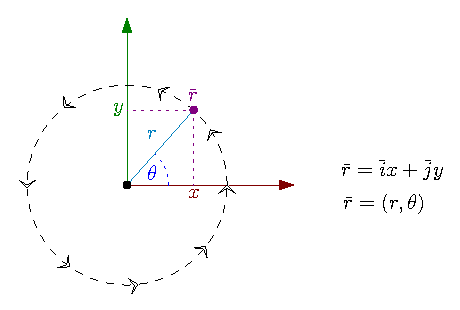
\includegraphics[width=0.5\textwidth]{images/motoCircUn.eps}
    \end{figure} 
\end{center}
Sia $\bar v$ la velocità, essendo il modulo costante, denoteremo $|\bar v|=v_0$. Si considera ora 
la velocità scalare $s$, di cui si ricorda 
$$ \frac{ds}{dt}=v_0$$
Inoltre, sapendo che $\frac{s}{R}=\theta$, si pone 
$$ \frac{ds}{R}=d\theta \implies \frac{ds}{dt}=R\cdot \frac{d\theta}{dt}=v_0$$
Denotiamo $\omega = \dfrac{d\theta}{dt}$, tale termine descrive la variazione dell'angolo nel tempo 
ed è denominato \textbf{velocità angolare}. Il fatto che la velocità dipenda dal raggio $R$, descrive il fatto 
che a parità di velocità angolare, un oggetto che si muove su un cerchio di raggio minore va meno veloce. 
$$ \frac{d\theta}{dt}=\omega \;\;\;\;\;\;\;\;\;\;\;\;\;\;\;
\frac{ds}{dt}=R\omega \;\;\;\;\; \;\;\;\;\;\;\;\;\;\;
v_0=R\omega$$
La velocità angolare si misura in radianti al secondo, essendo i radianti adimensionali, l'unità 
di misura è $\nicefrac{1}{s}=1 Hz$, detta anche \textit{frequenza}. Si può esprimere 
anche $\omega=\frac{2\pi}{t}$ dove $t$ rappresenta il tempo impiegato per fare un giro intero, 
detto anche \textit{periodo}. Si pone  la frequenza $\frac{1}{t}=\nu$ e si ha 
$$\frac{2\pi}{t} \nicefrac{1}{s}=2\pi\nu\ Hz$$
Si ha quindi la velocità angolare $\omega$, si vuole però rappresentare il vettore 
velocità $\bar v$, serve prima definire il vettore velocità angolare $\bar \omega$, ossia un vettore il cui modulo è 
uguale alla velocità angolare 
$$ |\bar \omega|=\omega = \frac{v}{R}$$
Il vettore $\omega$, essendo che deve rappresentare una rotazione, deve definire \begin{itemize}
    \item la velocità di rotazione 
    \item il piano di rotazione 
    \item il verso della rotazione 
\end{itemize}
Un piano, può essere definito dal suo \textit{vettore normale}, ossia il vettore ortogonale ai due 
vettori le cui combinazioni lineari generano tutti i punti del piano. Inoltre, il verso di tale vettore, 
definisce anche il verso di rotazione. 
$$\bar \omega \times \bar r = \bar v$$
rispetta infatti 
$$|\bar \omega \times \bar r| = |\bar v|\implies \omega R = v$$
Si ricordi che il vettore spostamento si muove sempre sul cerchio di raggio $R$, per questo 
$\bar r = R$.
\begin{center}
    \begin{figure}[h!]
        \centering
        \includegraphics[width=0.4\textwidth]{images/vetVelocitaAngolare.eps}
        \caption{vettore velocità angolare}
    \end{figure} 
\end{center}
Per convenzione, la rotazione avviene in senso antiorario intorno al vettore, se lo si osserva dal punto 
diretto dal suo verso.\begin{center}
    \begin{figure}[h!]
        \centering
        \includegraphics[width=0.4\textwidth]{images/dirVetAng.eps}
    \end{figure} 
\end{center}
Una volta stabilito il vettore velocità, si vuole trovare l'accelerazione, derivandola 
$$ \bar a = \lim_{\Delta t\rightarrow 0}\dfrac{\Delta \bar v}{\Delta t}$$
Definiamo $\Delta \theta$ l'angolo formato dal vettore $\bar r(t+\Delta t)$ con il vettore 
$\bar r(t)$, definisce la variazione dell'angolo nel tempo, è chiaro che se 
$\Delta t\rightarrow 0$ allora $\Delta \theta\rightarrow 0$.\acc 
Differentemente, il vettore $\Delta \bar v=\bar v(t+\Delta t)-\bar v(t)$, tende a puntare 
al centro del cerchio attorno a cui il punto rotea. Trovata la sua direzione, se ne vuole 
stabilire l'intensita, ossia il suo modulo $|\bar a|=a$.
\begin{center}
    \begin{figure}[h!]
        \centering
        \includegraphics[width=0.4\textwidth]{images/accAng.eps}
    \end{figure} 
\end{center}
Se $\Delta t$ tende a zero, l'arco di curva è approssimabile ad una retta fra i due punti, che 
sappiamo essere di lunghezza $|\Delta \bar r|=\Delta r$, inoltre, il rapporto fra quest'ultimo ed 
il raggio è proprio uguale all'angolo, quindi 
$$ \lim_{\Delta t \rightarrow 0}\frac{\Delta r}{R}=\Delta \theta $$
Inoltre, anche considerando il vettore $\Delta \bar v$, esso rispetto al vettore velocità 
permette di trovare il medesimo angolo 
$$ \lim_{\Delta t \rightarrow 0}\frac{\Delta \bar v}{v}=\Delta \theta $$
Quindi $$ |\Delta \bar v |= v\Delta \theta = \frac{\Delta r}{R}v$$
Indicando con $v$ il modulo di $\bar v$, si ha che 
$$ a=\lim_{\Delta t\rightarrow 0}\frac{\Delta v}{\Delta t}=
\lim_{\Delta t\rightarrow 0} \frac{v}{R}\frac{\Delta r}{\Delta t}$$
Appare come secondo termine proprio la derivata dello spostamento 
$$\lim_{\Delta t\rightarrow 0} \frac{v}{R}\frac{\Delta r}{\Delta t}= 
\frac{v}{r}(\lim_{\Delta t\rightarrow 0}\frac{\Delta r}{\Delta t})\implies  $$
\eqImportante{$|\bar a|=a=\frac{v^2}{R}=\omega^2R$}
\begin{center}
        \includegraphics[width=0.2\textwidth]{images/accelerazioneNormale.eps}
\end{center}
Si ricordi come il vettore accelerazione può essere scritto come somma di due componenti 
che rappresentano l'accelerazione tangenziale, ossia la variazione del modulo della velocità, e 
\textbf{l'accelerazione normale}, che descrive il variare della direzione della velocità. Nel 
caso del moto rettilineo uniforme, l'accelerazione ha componente tangenziale nulla, è solo 
normale e diretta verso il centro del cerchio, ed ha intensità $\frac{v^2}{R}$.\acc 
Quando un moto di un punto $\bar r$ segue una traiettoria curva (ma non circolare uniforme), preso un istante 
fissato $t_0$, l'accelerazione normale è diretta verso il centro del cerchio che approssima la curva 
nell'istante dato e che contenga $\bar r(t_0)$, come mostrato in figura \ref{cerchioOsculante}.
\acc 
A tal punto è possibile descrivere un moto qualsiasi definendo la sua accelerazione normale 
e tangenziale. Il moto circolare uniforme è il particolare caso in cui l'accelerazione 
tangenziale è nulla. $$ \begin{cases}
    \bar v(t) = \bar \omega(t) \times \bar r(t)   \\ 
    \bar a_t(t)  = \frac{d\bar \omega}{dt}(t)|\bar r|(t) \text{ accelerazione tangenziale} \\ 
    \bar a_n(t) = \frac{\bar v(t)^2}{\bar r(t)}\text{ accelerazione normale}
\end{cases}$$
\begin{center}\begin{figure}[h!]
    \centering
    \includegraphics[width=0.7\textwidth]{images/cerchioOsculante.eps}
    \caption{Cerchio osculatore}
    \label{cerchioOsculante}
\end{figure} \end{center}
\subsection{Moto Armonico}
Il moto armonico vuole descrivere il comportamento oscillatorio e periodico di un punto. Si può 
descrivere come la proiezione su uno degli assi del moto circolare uniforme. 
$$ x(t)=R\cos(\theta(t))=R\cos(\omega t)$$
\begin{center}\begin{figure}[h!]
    \centering
    \includegraphics[width=0.9\textwidth]{images/armonica.eps}
    \caption{$x(t)=R\cos(\omega t)$}
    \label{cerchioOsculante}
\end{figure} \end{center}
La costante $R$ si chiama \textit{ampiezza} del moto, mentre $\omega$ si chiama \textit{pulsazione}.
La funzione $x$ del moto è armonica di periodo $T$, ossia $x(t+T)=x(t)$. Essendo che l'argomento della  funzione  
trigonometrica deve variare di $2\pi$ si ha 
$$\omega(t+T)-\omega t = 2\pi \implies \omega = \frac{2\pi}{T}=2\pi\nu$$
Si definisce $\nu=\frac{1}{T}$ una nuova grandezza denominata \textit{frequenza} di moto.
\acc Si vuole trovare la velocità, ossia 
$$ v(t)=\frac{d}{dt}R\cos(\omega t)=-R\omega\sin(\omega t)$$
La velocità massima si ha in $-R\omega\sin(\omega t)=0\implies \sin(\omega t)=0$, ossia nei punti 
in cui $x$ incontra l'asse delle ascisse. L'accelerazione vale 
$$ a=\frac{dv}{dt}=\frac{d}{dt}-R\omega\sin(\omega t)=-R\omega^2\cos(\omega t)=-\omega^2x(t)$$
Si noti come l'accelerazione dipende dalla posizione, la sua forza è proprio opposta ad essa, 
si dice infatti che il moto oscillatorio è dettato da una \textit{forza di richiamo}.
\flowerLine
\section{Moti Relativi}
La velocità è relativa, le caratteristiche di un punto sono legate al suo sistema di riferimento, e 
al suo sistema di coordinate. Il moto di un punto può essere osservato diversamente da due sistemi 
di riferimento differenti.\acc 
Si considerino due sistemi di riferimento $O$ e $O'$, per semplicità, siano il piano cartesiano, di 
cordinate (rispettivamente) $x,y$ e $x',y'$. Supponiamo inoltre, che all'origine dei tempi, essi 
si trovino nella stessa posizione, e che il sistema $O'$ si muova con velocità costante $\bar v = (v_0^x,0)$.
\begin{center}
    \includegraphics[width=0.6\textwidth]{images/sistemiRif.eps}
    \end{center}
Vi è poi un punto nello spazio, che secondo il sistema di riferimento $O$, è fermo, ed ha cordinate $x_0$. 
Si vuole trovare tale punto nel sistema di riferimento $O'$. Tale sistema, si allontana da $O$ ad una 
velocità costante $v_0^x$, intuitivamente, avendo $O$ una velocità "assoluta" nulla,
 vedrà allontanarsi il punto $x_0$ a velocità $v_0^x$. La velocità è de facto relativa al sistema di riferimento, 
 non esiste quindi una velocità assoluta, ma si sceglie arbitrariamente un sistema di riferimento 
 da considerare fisso, l'altro sistema sarà detto "mobile", ed il moto in esso, sarà 
 detto "relativo". 
 $$x_0'=x_0-v_0^xt$$
In generale, la formula per il \textit{passaggio di coordinate} è la seguente
$$\begin{cases}
    x\\ y\\ z\\ t
\end{cases} \implies \begin{cases}
    x' = x-v_0^x t\\ 
    y' = y-v_0^y t\\ 
    z' = z-v_0^z t\\ 
    t'=t \text{ il tempo è assoluto}
\end{cases}$$
Dove $\bar v_0=(v_0^x,v_0^y,v_0^z)$ è la velocità del secondo sistema di riferimento.
\acc 
Il moto del punto nel sistema di riferimento fisso, visto dal sistema di riferimento relativo, è 
detto \textit{moto di trascinamento}, nell'esempio trattato, tale moto è una traslazione, si dice 
infatti moto di trascinamento traslatorio. Denoteremo $$ \begin{matrix}
    \bar v_a \text{ velocità assoluta }\\ 
    \bar v_r \text{ velocità relativa }\\ 
    \bar v_t \text{ velocità traslatoria }
\end{matrix}$$ 
$$\bar v_a(t)=\bar v_r(t)+\bar v_t \ \ \ \ \ \textbf{composizione delle velocità}$$ 
Ne consegue che 
$$a_a(t)=\frac{d}{dt}v_a(t)=\frac{d}{dt}v_r(t)+v_t=a_r $$ 
Se la velocità è costante, l'accelerazione assoluta, come quella relativa risulterà nulla, in tale 
configurazione il sistema è detto \textbf{inerziale}.\acc 
\textbf{Esempio (nuotatore)} : Si consideri un fiume in cui una corrente spinge chiunque vi sia all'interno 
con una velocità costante $\bar v_t$, un nuotatore, vuole attraversare il fiume in linea retta, 
la sua velocità è $\bar v_r$, tale che $|\bar v_r|>|\bar v_t|$.\acc 
Partendo da una sponda, il nuotatore deve decidere in che direzione nuotare per far si che 
la sua velocità si bilanci con la corrente del fiume, facendo risultare il suo moto 
assoluto $\bar v_a$ in modo che attraversi il fiume in linea retta.
\begin{center}
    \includegraphics[width=0.6\textwidth]{images/nuotatore.eps}
\end{center}
Si vuole trovare l'angolo $\alpha$ fra la velocità relativa e quella di trascinamento per far 
si che la velocità assoluta sull'asse delle parallelo alle sponde sia nulla.
$$ v_r \sin(\alpha)=- v_t \implies \alpha = -\arcsin(\frac{v_t}{v_r}) $$ 
Si consideri ora un sistema non inerziale, ossia in cui la velocità di trascinamento dipende dal tempo 
$$\bar v_a(t) = \bar v_r(t) + \bar v_t(t) $$
Ne consegue che l'accelerazione di trascinamento non è nulla. 
$$\bar a_a = \bar a_r + \bar a_t + \bar a_c $$
Il termine $\bar a_c$ risulta ambiguo, essa è detta \textit{forza di Coriolis}, è una 
forza apparente (si tratteranno in seguito), e si manifesta 
quando il sistema di riferimento sta ruotando, si ha che 
$$\bar a_c = 2\bar \omega \times \bar v_r $$
Dove $\bar \omega$ è il vettore velocità angolare del sistema in rotazione. Un tipico esempio di 
manifestazione di tale accelerazione è il seguente : Ci si trova su una giostra che sta ruotando, 
si lancia un oggetto davanti a se, la traiettoria di tale oggetto non sarà dritta come 
voluto, ma curverà verso l'esterno della giostra.\begin{center}\begin{figure}[h!]
    \centering
    \includegraphics[width=0.3\textwidth]{images/Coriolis.eps}
    \caption{Forza di Coriolis}
    \label{fig:Coriolis}
\end{figure} \end{center}
\flowerLine
\section{Esercizi sul Punto Materiale}
\subsubsection{Esercizio 1)}
Un punto materiale si muove su una traiettoria rettilinea con un accelerazione 
$a=-4t\nicefrac{m}{s^2}$, all'istante $t=0$, ha una velocità iniziale di $v_0=2\nicefrac{m}{s}$. 
Quanto spazio percorrerà prima di fermarsi?\\ 
Si vuole trovare la legge della velocità 
$$v(t)=\int_0^t a  \ dt + v_0=-2t^2+v_0$$
La legge oraria dello spostamento sarà 
$$ s(t)=\int_0^t v \ dt = v_0t-\frac{2}{3}t^3$$
Il punto si fermerà quando la velocità sarà uguale a zero, sia $t_1$ l'istante in cui ciò avviene 
$$ v(t_1)=0\implies -2{t_1}^2+v_0=0\implies t_1=\sqrt{\frac{v_0}{2}}$$
All'istante $t_1$, lo spazio percorso sarà 
$$ s(t_1)=v_0t_1-\frac{2}{3}{t_1}^3=
v_0\sqrt{\frac{v_0}{2}}-\frac{2}{3}{(\sqrt{\frac{v_0}{2}})}^3$$Sapendo che $v_0=2\nicefrac{m}{s}$
$$
2\sqrt{\frac{2}{2}}-\frac{2}{3}{(\sqrt{\frac{2}{2}})}^3=\frac{4}{3} m
$$
\subsubsection{Esercizio 2)}
All'istante $t=0s$ un punto materiale parte da fermo e si mette in moto su una traiettoria circolare 
di raggio $R=225m$, continua il suo moto fino all'istante $t_1=10s$, la velocità del punto, cresce 
linearmente con il tempo, e all'istante $t_1$ lo spazio percorso è di $150m$. Si determini il modulo dell'accelerazione 
all'istante $t_1$.\\ 
Se la velocità cresce linearmente con il tempo, il suo modulo sarà del tipo 
$$ v(t)=v(0)+a_tt=0+a_tt=a_tt$$
dove con $a_t$ si definisce l'accelerazione tangenziale. La legge dello spostamento  è 
$$s(t)=s(0)+\int_0^ta_ttdt=\frac{1}{2}a_tt^2$$
L'accelerazione tangenziale è quindi 
$$ a_t=2\frac{s(t)}{t^2}$$
All'istante $t_1$, l'accelerazione tangenziale sarà 
$$a_t(t_1) = 2\frac{s(t_1)}{(t_1)^2}=2\frac{150}{(10)^2}=3\nicefrac{m}{s^2}$$
È nota la formula dell'accelerazione normale 
$$ a_n(t_1)=\frac{v(t_1)^2}{R}=\frac{{v(10)}^2}{225}=\frac{{3\cdot 10}^2}{225}=\frac{900}{225}=4\nicefrac{m}{s^2}$$
L'accelerazione sarà quindi 
$$a(t_1)=\sqrt{a_t^2(t_1)+a_n^2(t_1)}=\sqrt{9+16}=5\nicefrac{m}{s^2}$$ 
\subsubsection{Esercizio 3)}
Un aereo vola con velocità costante $v_0$, seguendo una rotta rettilinea inclinata verso
 il basso di un angolo $\alpha$ rispetto all'orizzonte. Se il pilota volesse
  centrare un bersaglio a terra sganciando una massa puntiforme da una quota $h$,
   a quale distanza $d$ dal bersaglio dovrebbe sganciarla?\acc
Ci si vuole assicurare che, la bomba, la cui velocità dipenderà da quella iniziale data 
dall'aereo, e dall'accelerazione di gravità, incroci l'asse delle ascisse nel punto del bersaglio, che 
dista $d$ dall'aereo. Si vuole far si che tale bomba percorrà una distanza $d$ sull'asse delle ascisse, ed 
una distanza $h$ sull'asse delle ordinate. La velocità $\bar v=(v_x,v_y)$ di tale bomba risulta essere 
$$\begin{cases}
    v_x(t)=v_0\cos\alpha\\ 
    v_y(t)=v_0\sin\alpha+gt
\end{cases} $$
   \begin{figure}[h!]
    \centering
    \includegraphics[width=0.6\textwidth]{images/es3.eps}
    \caption{schema esercizio 3}
\end{figure}
Lo spostamento sarà rispettivamente 
$$ \begin{cases}
    x(t)=v_0\cos\alpha t\\ 
    y(t)= v_0\sin\alpha+\dfrac{gt^2}{2}
\end{cases}$$
Sia $t^*$ l'istante in cui la bomba colpisce il bersaglio 
$$ x(t^*)=d=v_0\cos\alpha t^*$$ 
$$ y(t^*)=h= v_0\sin\alpha+\frac{g{t^*}^2}{2}$$
Si risolve il sistema per trovare tale istante 
$$ \begin{cases}
    v_0\sin\alpha+\dfrac{g{t^*}^2}{2}=h\\ 
    v_0\cos\alpha t^=d*
\end{cases}\implies 
t^*=-\frac{v_0}{g}\sin\alpha+\sqrt{\frac{v_0^2}{g^2}\sin^2\alpha+\frac{2h}{g}}$$
Quindi 
$$ 
d=v_0\cos\alpha\Bigg(
    -\frac{v_0}{g}\sin\alpha+\sqrt{\frac{v_0^2}{g^2}\sin^2\alpha+\frac{2h}{g}}\     
\Bigg)
$$
\chapter{Dinamica}
\section{Forze}
Newton considerò il principio di inersia e lo fece suo, definì i 3 principi della dinamica
\subsubsection{Primo Principio}
Lo stato naturale di un corpo in assenza di perturbazioni è quello di moto rettilineo uniforme 
\subsubsection{Secondo Principio}
\defi{} Si definisce \textit{quantità di moto} il prodotto della velocità di un corpo per la sua massa 
$$ \bar p = m\cdot \bar v$$ 
Definiamo \textit{forza} il fenomeno capace di perturbare i corpi, ed equivale alla derivata rispetto al tempo 
della quantità di moto. 
\eqImportante{$\bar F = \dfrac{d\bar p}{dt}$} 
\subsubsection{Terzo Principio}
\textit{Ad ogni azione corrisponde una reazione uguale e contraria}. Quando un corpo in un punto $A$ esercita una forza 
su un altro corpo in un punto $B$, esso subisce una reazione uguale in intensità e diretta lungo la 
congiungente dei due punti.\begin{center}
    \includegraphics[width=0.6\textwidth]{images/terzoPrincipio.eps}
\end{center}
$\bar F$ modellizza una generica forza, la massa $m$ che compare nella sua formula è detta 
massa inerziale. Una forza di cui risente ogni abitante sulla terra è la forza peso 
$$ \bar F \equiv m_g\bar g$$
dove $m_g$ è detta massa gravitazionale, nel caso in cui dovesse coincidere con quella 
inerziale, si avrebbe che $\bar a = \bar g$. La legge di gravitazione universale, da cui si ricava la 
forza peso, descrive la forza che attrae un corpo di massa $m$ verso un altro di massa $M$
$$ \bar F = -G\frac{mM}{|\bar r|^2}\bar r$$
Dove $\bar r$ è il vettore che congiunge i due corpi. La forza di gravità è quindi proporzionale alle masse dei 
corpi, e diminiusce con l'aumentare della distanza al quadrato.
\subsection{Forza Elastica}
Un'altra forza presente nella vita quotidiana è quella elastica, modellizza macroscopicamente, il comportamento 
di una molla. $$ \bar F = k(\bar r - \bar r_0)$$
Dove $\bar r$ è la posizione del corpo che subisce la forza, $\bar r_0$ è uno specifico punto nello spazio 
detto equilibrio, e $k$ è una costante detta \textit{costante di elasticità}, scriviamo nel caso unidimensionale 
$$ F=k\cdot(x-x_0)$$
Più ci si allontana dal punto di equilibrio, più la forza aumenta, ed essa è nulla proprio in 
tale punto. Si vuole descrivere il moto di un corpo soggetto a forza 
elastica. Per semplicità, si consideri $x_0=0$
$$ \begin{matrix}F=-kx\\ \\ F=m\dfrac{d^2x}{dt^2} 
\end{matrix}\implies 
\frac{d^2x}{dt^2}{}+\frac{k}{m}x=0$$
La soluzione dell'equazione differenziale, ossia la legge oraria di un corpo soggetto a forza elastica, 
è la seguente 
$$ A\cos(\omega_0t+\phi)$$
$A$ e $\phi$ sono due costanti che dipendono dalle condizioni iniziali $x(0)$ e $v(0)$. La relazione è la seguente 
$$ x(0)=A\cos\phi$$
La legge della velocità si ottiene derivando $x$
$$ v(t)=-A\omega_0\sin(\omega_0t+\phi)$$
Quindi 
$$ v(0)=-A\omega_0\sin\phi\implies \frac{v(0)}{\omega_0}=-A\sin\phi$$
Si considerino i quadrati 
$$\begin{cases}
    x(0)^2=(A\cos\phi)^2\\ 
   ( \frac{v(0)}{\omega_0})^2=(-A\sin\phi)^2
\end{cases}\implies \begin{cases}
    \phi=-\arctan(\dfrac{v(0)}{w_0x(0)})\\ 
    A = \sqrt{x(0)^2+(\dfrac{v(0)}{w_0})^2}
\end{cases}$$
\subsection{Reazione Normale}
Si consideri un corpo di massa $m$ posto su un piano inclinato di un angolo $\alpha$ rispetto 
l'orizzonte (il cui attrito è nullo). Il corpo è soggetto alla forza peso, perché allora non sfonda il piano cadendo verso il 
centro della terra? Esso è soggetto ad una reazione normale $\bar{R_n}$, ossia una forza la cui direzione è la normale 
della superficie su cui poggia. Il piano costituisce un vincolo, si parla infatti di \textit{reazione vincolare}.
\begin{center}
    \includegraphics[width=0.5\textwidth]{images/reazionenormale.eps}
\end{center}
Il corpo, sarà soggetto alla somma delle due forze 
$$ \bar F = m\bar a = m\bar g + \bar{R_n}$$
Tenedrà quindi ad accelerare lungo l'asse del piano, si vuole trovare il moto di tale corpo. Consideriamo un 
sistema di riferimento in cui l'asse delle $y$ è parallela alla reazione normale, e l'asse delle $x$ 
forma un angolo $\alpha$ con l'orizzonte.
\begin{center}
    \includegraphics[width=0.55\textwidth]{images/reazionenormale2.eps}
\end{center}
Si vuole quindi trovare l'accelerazione lungo $x$, bisogna proiettare entrambe le forze su tale asse. 
Come si può vedere dall'immagine, la reazione normale non esercita alcuna forza su tale asse, ma esclusivamente sull'asse 
delle $y$ 
$$ |\bar R_n|=\sin\alpha|\bar R_n| $$
in particolare, una forza che controbilancia quella peso, e fa si che il suo spostamento sull'asse $y$ sia nullo. 
$$ -m|\bar g|\sin \alpha +|\bar R_n|=0$$
Lungo l'asse delle ascisse, la proiezione della forza sarà 
$$ F_x=mg\cos\alpha\implies ma_x=mg\cos\alpha=a_x=g\cos\alpha$$
A questo punto si può trovare il moto del corpo sull'asse delle $x$
$$ x(t)=\frac{1}{2}g\sin\alpha t^2$$
\subsection{Attrito}
Nell'esempio precedente del piano inclinato si è trascurato l'attrito, tale forza si manifesta a seguito di uno 
strusciamento fra due corpi, ed è dovuta all'asperità dei materiali a livello microscopico. È fondamentale considerarlo 
quando si devono calcolare le forze in una situazione reale.\\
\begin{figure}[h!]
    \centering
    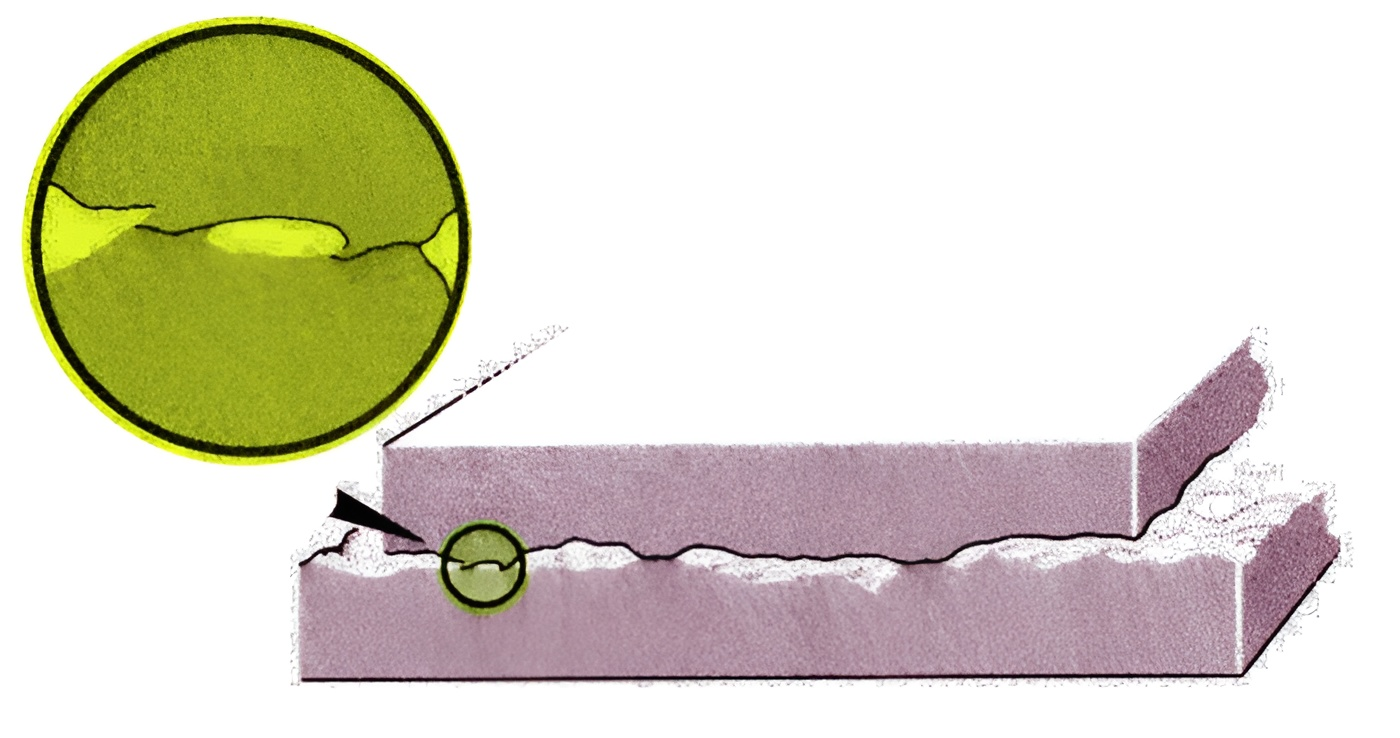
\includegraphics[width=0.45\textwidth]{images/attrito}
    \caption{asperità dei materiali}
\end{figure}\acc
L'attrito si presenta sotto due aspetti\begin{itemize}
    \item \textbf{attrito statico} : Forza esercitata su un corpo fermo su una superficie, che subisce una forza 
    \item \textbf{attrito dinamico} : Forza esercitata su un corpo in movimento che si sposta strisciando su una superficie
\end{itemize}
La modellizzazione dell'attrito prevede tale suddivisione, quando un corpo su una superficie subisce 
una forza $\bar F$, è anche soggetto ad una forza di attrito statico $\bar F_s$, essa si oppone alla prima, 
de facto è uguale in intensità e direzione, ma il verso è contrario. Se la forza applicata varia, l'attrito 
varierà con essa.\acc 
In una situazione reale però, quando si spinge un oggetto, aumentando l'intensità il corpo inizierà a muoversi, 
esiste quindi una forza di soglia sotto il quale l'attrito statico vale, una volta raggiunta tale soglia, 
il corpo si muoverà, e sarà soggetto ad attrito dinamico. In generale, tale soglia è descritta da 
$$ F_s\le \mu_s\cdot R_n$$
Dove $R_n$ è il modulo della reazione normale che subisce il corpo che poggia sulla superficie, e 
$\mu_s$ è il \textit{coefficente di attrito statico}, e dipende dal materiale dei corpi. Essendo tale attrito 
proporzionale alla reazione normale, risulta chiaro ora il perché gli oggetti posti su un piano inclinato necessitano
 di meno forza per essere spostati.\acc 
 Quindi $F_s$ è sempre uguale alla forza applicata sul corpo ma contraria di verso finché il suo modulo è minore 
 di $\mu_s\cdot R_n$. Se tale modulo è maggiore, allora il corpo sarà soggetto ad un 
 attrito dinamico $\bar F_d$
 $$ \bar F_d = -\mu_d\cdot R_n\cdot \bar \tau$$
$\mu_d$ è il coefficiete di attrito dinamico, tipicamente, per uno stesso materiale $\mu_s>\mu_d$. $\tau$ è il 
versore parallelo alla velocità del corpo che subisce tale attrito. La decelerazione che subirà 
il corpo che si muove su una superficie sarà
$$ m\bar a = -\mu_dR_n\bar \tau\implies m\bar a = -\mu_dmg\bar \tau \implies |\bar a| = -\mu_d g$$
Nella formula, si è sostituito $R_n$ ad $mg$, in quanto il modulo di tali forze è lo stesso, come già visto 
$$ R_n-mg=0$$
\begin{center}
    \includegraphics[width=0.5\textwidth]{images/attritoDinamico.eps}
\end{center}
Si noti come la decelerazione subita non dipende dalla massa del corpo, ma esclusivamente dalla reazione 
normale e dalla costante di attrito dinamico. Si ricavano le leggi della velocità e dello spostamento (nel caso 
unidimensionale) 
$$ v=v_0-\mu_dgt$$ 
$$ x=v_0t-\frac{1}{2}\mu_dgt^2$$
Il corpo si fermerà nell'istante $t_1$ in cui $v(t_1)=0$
$$ v(t_1)=0\implies v_0-\mu_dgt_1=0\implies t_1=\frac{v_0}{\mu_dg}$$
E lo spazio percorso sarà 
$$ x(t_1)=v_0t_1--\frac{1}{2}\mu_dg{t_1}^2=
v_0(\frac{v_0}{\mu_dg})-\frac{1}{2}\mu_dg{(\frac{v_0}{\mu_dg})}^2=\frac{v_0^2}{2\mu_dg}
$$
\subsubsection{Misuratore di Attrito}
Il seguento esempio, mostra com'è possibile sfruttare un piano inclinato, la cui inclinazione 
$\alpha$ è variabile, per misurare la costante di attrito statico e dinamico di un corpo. Supponiamo quindi, di posare un 
corpo su tale piano, la cui inclinazione iniziale è nulla. Cominciando a sollevare il piano (variando $\alpha$), il corpo 
rimarrà in uno stato di quiete, finché non avrà forza a sufficienza da superare l'attrito statico. Tale 
soglia equivale a $$mg\sin\alpha $$
L'attrito statico è limitato da tale valore, sia $\alpha_1$ il massimo valore dell'angolo per cui 
il corpo non si muove, in tal caso si ha 
$$ mg\sin\alpha_1=\mu_smg\cos\alpha_1\implies\mu_s=\tan\alpha_1$$
Si consideri adesso l'insieme dei valori $\alpha>\alpha_1$, per cui il corpo si muove ed è soggetto 
ad attrito dinamico. In particolare la sua forza sarà 
$$ma=m\sin\alpha-\mu_dR_n $$
Si varia l'angolo $\alpha$ per trovare il punto in cui il corpo non subisce più accelerazione, ossia $a=0$. Sia 
$\alpha_2$ tale valore 
$$ mg\sin\alpha_2-\mu_dR_n=0$$
Si ricordi $R_n=mg\cos\alpha_2$
$$ mg\sin\alpha_2=\mu_dmg\cos\alpha_2\implies \mu_d=\tan\alpha_2$$
\flowerLine 
\section{Impulso e Lavoro}
Si è visto come la dinamica permette di descrivere le equazioni 
del moto tramite le forze, in certi casi, non è chiara l'evoluzione 
nel tempo di una determinata forza, ma è comunque possibile 
avere informazioni globali sul suo comportamento grazie ad un
 integrazione. Si consideri l'integrazione della forza nel tempo in un dato 
 intervallo $[t_1,t_2]$
 $$ \int_{t_1}^{t_2}\bar F dt$$
 Le dimensioni sono espresse in $mv$, massa per velocità. Precisamente 
\begin{eqnarray}
    \int_{t_1}^{t_2}\bar Fdt =\\ 
    \int_{t_1}^{t_2} = m\dfrac{d\bar v}{dt}dt =\\ 
    m\int_{ \bar v_1}^{ \bar v_2}d\bar v = m\bar v_2-m\bar v_1=\\
    m(\bar \bar v_2-\bar v_1)
\end{eqnarray}
Risulta essere la variazione della quantità di moto, tale grandezza 
è nota come \textbf{impulso}
\eqImportante{$I=\Delta\bar p$}
Se la forza non è nota analiticamente, è possibile 
considerare la \textit{forza media} come il rapporto fra l'impulso 
e la variazione nel tempo, sia $t_2=t_1+\Delta t$
$$ \frac{I}{\Delta t}=\frac{\Delta \bar p}{\Delta t}
=\frac{1}{\Delta t}\int_{t_1}^{t_2}\bar F dt$$
Risulta utile nella descrizione dei fenomeni che agiscono in 
un breve lasso di tempo con una certa intensità, come gli urti, dette 
forze impulsive.\acc 
\textbf{Esempio} : Quando si vuole inserire un chiodo in una tavola di legno, si colpisce 
con un martello il chiodo. Se provassimo a salire sul chiodo applicheremmo una forza pari al nostro peso, che è 
di gran lunga superiore al peso del martello, ciònonostante, il chiodo non entrerebbe nella fessura, la forza non sarebbe 
necessaria.\acc 
Quanta forza viene trasmessa allora al colpo del chiodo sul martello? Supponiamo che il chiodo non assorba 
forza, e la rifletta completamente, ciò significa che rifletterà una quantità di moto pari alla quantità 
di moto applicata. Sia $mv$ la quantità di moto iniziale, il martello una volta colpito il chiodo avrà una 
quantità di moto $-mv$, la differenza sarà quindi $\Delta p=2mv$.\begin{center}
    \includegraphics[width=0.7\textwidth]{images/chiodo.eps} 
\end{center}
Supponiamo che il martello pesi $0.5kg$, che arrivi sul chiodo ad una velocità pari a $5\frac{m}{s}$, la sua quantità 
di moto sarà quindi $0.5\cdot 5=2.5kg\frac{m}{s}$. L'evoluzione della forza nel tempo in cui colpisce il chiodo non è 
nota, ma è possibile stabilire la forza media tramite l'espressione $\frac{\Delta p}{\Delta t}$, supponiamo che 
il lasso di tempo in cui il martello colpisce il chiodo sia di $10^{-3}s$. Allora la forza media sarebbe 
$$ \frac{2.5}{10^{-3}}kg\frac{m}{s^2}=2500N$$
\subsection{Lavoro ed Energia Potenziale}
Quindi l'impulso deriva dall'integrazione della forza rispetto al 
tempo, essa può essere derivata anche rispetto allo spazio.
Supponiamo che vi siano una curva che unisce i punti $A$ e $B$, 
definiamo \textbf{lavoro} l'integrale 
$$ L=\int_A^B\bar Fd\bar s$$
Dove $d\bar s$ rappresenta lo spostamento infinitesimo lungo la curva, e 
$\bar Fd\bar s$ è il prodotto scalare, di cui 
$$ |\bar Fd\bar s|=Fds\cos\theta$$\begin{center}
    \includegraphics[width=0.4\textwidth]{images/lavoro.eps}
\end{center}
Le dimensioni del lavoro sono $ml^2t^{-2}$, l'unità di misura 
è il \textit{joule} e si denota $J$. Il lavoro può 
essere descritto come segue (si assuma che la massa della forza 
sia costante) 
\begin{eqnarray}
    L=\int_A^B\frac{dm\bar v}{dt}d\bar s = \\ 
    \int_A^Bmd\bar v\frac{d\bar s}{dt}
\end{eqnarray}
essendo $\frac{d\bar s}{dt}=\bar v$
\begin{eqnarray}
    \int_A^Bm\bar vd\bar v
\end{eqnarray}
Tralasciando momentaneamente l'espressione del lavoro, si noti come 
\begin{eqnarray}
    \bar v \cdot \bar v =  v^2 \text{ differenziando}\\ 
    \bar vd\bar v+\bar d\bar v\bar v=d v^2 \implies \\ 
    2d\bar v \cdot \bar v =d\bar v \bar v = \frac{1}{2}dv^2
\end{eqnarray}
quindi, tornando al lavoro
$$
    \int_A^Bm\bar vd\bar v=\int_{v_1^2}^{v_2^2}dv^2
$$
Dove $v_1$ e $v_2$ sono le velocità, rispettivamente, in $A$ ed 
in $B$ (velocità iniziale e velocità finale)$$ 
\int_{v_1^2}^{v_2^2}dv^2=\frac{1}{2}mv_2^2-\frac{1}{2}mv_1^2
$$
Definiamo $T=\frac{1}{2}mv^2$ \textbf{energia cinetica}, quindi 
$$ L=\Delta T$$
Il lavoro è \textit{la variazione dell'energia cinetica}.
\subsection{Forze Conservative}
Vediamo ora una particolare classe di forze, ossia quelle 
\textit{conservative}.\acc 
\defi{} Una forza è detta \textbf{conservativa} se il lavoro 
valutato su una curva fra due punti $A$ e $B$ è indipendente dal 
percorso considerato. Siano $\delta_1$ e $\delta_2$ due curve 
differenti, che però hanno entrambe $A$ e $B$ come punti di 
congiunzione, $\bar F$ è conservativa se 
$$ \int_{\delta_1}\bar Fd\bar s=\int_{\delta_2}\bar Fd\bar s$$
Un esempio di forza conservativa è la forza di gravità
 $\bar F_g=m\bar g$, che riscreveremo $-mg\hat y$
 $$ L=\int_{A}^B -mg\hat y d\bar s = -mg\int_A^B \hat y d \bar s$$
Si consideri il termine $\hat y d\bar s$, il modulo di $d\bar s$ 
è infinitesimo, mentre il modulo di $\hat y$ è 1. Il loro prodotto 
scalare non è altro che lo spostamento infinitesimo lungo l'asse $y$
$$
-mg\int_A^B \hat y d \bar s = -mg\int_{y(A)}^{y(B)}dy
$$
Definiamo $y(A)$ come la coordinata $y$ del punto $A$,
analogo per $y(B)$.\begin{center}
    \includegraphics[width=0.4\textwidth]{images/gravitaConservativa.eps}
\end{center}
$$ -mg\int_{y(A)}^{y(B)}dy=mgy(A)-mgy(B)$$
Definiamo $mgy=U(y)$ \textbf{energia potenziale}
$$ L=-mg\int_{y(A)}^{y(B)}dy=U(A)-U(B)=-\Delta U$$
\begin{quote}
    Nelle forze conservative, il lavoro su una curva che congiunge i punti $A,B$ è pari alla differenza
     dell'energia potenziale calcolata sui due punti.
\end{quote}
L'energia potenziale $U$ è definita anche per le altre forze, non esclusivamente 
per la forza di gravità, che in tal caso è servita come esempio. La gravità 
è una forza \textit{uniforme}\begin{quote}
    tutte le forze uniformi sono conservative
\end{quote}
Anche la forza gravitazionale definita da Newton è conservativa 
$$ \bar F_G=-G\frac{Mm}{r^2}\hat r$$
Dove $\hat r$ è il versore che va dal corpo di massa $m$ a quello di massa $M$, ed $r$ è la distanza fra i due corpi. Tale 
forza è detta \textit{centrale}, in ogni punto è diretta verso un punto $O$, l'intensità dipende 
solamente dalla distanza $r$ dal puntoi. Il lavoro su una curva 
che congiunge i punti $A,B$ risulta essere 
$$ \int_A^B\bar F_Gd\bar s=\int_A^B-G\frac{Mm}{r^2}\hat rd\bar s=
-GMm\int_A^B\frac{\hat r}{r^2} d\bar s$$
$\hat r$ ed $r^2$ non possono essere portati fuori dall'integrale dato che sono variabili e dipendono dalla 
posizione. Sia $OP$ il vettore che va dal punto $P$, posizione del corpo soggetto alla forza, all'origine della forza $O$, ossia 
il vettore di lunghezza $r$. In tal caso si ridefinisce $\hat r = \dfrac{OP}{|OP|}$. \acc 
Sia $F_G(r)$ il modulo della forza, esso dipende da $r$, tale che 
$$ \bar F_G(r)=F_G(r)\hat r$$
Si consideri un percorso qualsiasi $C$ che congiunga due punti $P_1$ e $P_2$, in corrispondenza di uno 
spostamento infinitesimo $d\bar s$ lungo tale percorso a partire da una posizione $P$, 
il lavoro infinitesimo sarà 
$$ dL=\bar F_Gd\bar s = F_G(r)dr$$
Dove $dr$ è la proiezione di $d\bar s$ su $OP$. 
$$ \hat r \cdot d\bar s=dr$$ 
\begin{center}
    \includegraphics[width=1\textwidth]{images/forzaCentrale.eps}
\end{center}
$$ 
-GMm\int_A^B\frac{\hat r}{r^2} d\bar s=
-GMm\int_{r_A}^{r_B}\frac{dr}{r^2}
$$
Dove $r_A$ ed $r_B$ sono le distanze dall'origine dei punti $A$ e $B$
$$-GMm\int_{r_A}^{r_B}\frac{dr}{r^2}=GMm\frac{1}{r_B}-GMm\frac{1}{r_A} $$
$$ U(r)=-\frac{GMm}{r} \ \  \textbf{ energia potenziale gravitazionale}$$
Inoltre 
$$ \lim_{r\rightarrow \infty}-\frac{GMm}{r}=0\implies U(\infty)=0$$
La forza di gravitazione a distanza infinita non compie lavoro.\begin{center}
    \begin{tikzpicture}[scale=1, transform shape]
		\begin{axis}[
		ymin=-10,
		ymax = 10,
		xmin=-10,
		xmax = 10,
		axis lines = center,
		xtick distance=500, ytick distance=500,
		grid style=dashed,
		ymajorgrids=true,
		xmajorgrids=true,
		xlabel = \(r\),
		ylabel = {\(U(r)\)},
		]
		%Below the red parabola is defined
		\addplot [
		domain=0:10,
		samples=100,
		color=blue,
		]
		{-5/x};
		\end{axis}
		\end{tikzpicture}
\end{center}
Anche la forza elastica è conservativa, consideriamo il caso unidimensionale (per semplicità, il punto di equilibrio 
è 0)
 $$ \bar F = -kx\hat x$$
 $$L=-k\int_{x_1}^{x_2}x\hat x d\bar s =  -k\int_{x_1}^{x_2}xdx=\frac{1}{2}k(x_1^2-x_2^2)$$
 $$ U(x)=\frac{1}{2}kx^2 \ \  \textbf{ energia potenziale elastica}$$
 Abbiamo definito il lavoro come 
 $$ L=\Delta T$$
 Ed il lavoro per le forze conservative come 
 $$L=-\Delta U$$
Perché le forze si dicono \textit{conservative}? Se una forza è conservativa, si ha 
$$ \Delta T+\Delta U = 0 \implies \Delta(T+U)=0$$
Si pone $E_{m}=T+U$, essa è detta \textbf{energia meccanica}, quindi 
$$ \Delta E_m=0$$
Il nome "conservativo" deriva dal fatto che tali forze \textit{conservano l'energia meccanica}, infatti 
la variazione di essa è nulla.\acc 
Si vuole calcolare l'energia meccanica totale di un corpo di massa $m$ che si trova in un orbita circolare 
di un pianeta di massa $M$ a distanza $R$, l'energia meccanica è la somma dell'energia potenziale e dell'energia 
cinetica. $$ U=-\frac{GmM}{R}\ \ T=\frac{1}{2}mv^2=\frac{GMm}{2R}\implies E_{mecc}=\frac{GMm}{2R}-\frac{GmM}{R}=-\frac{GmM}{2R}$$
\defi{( velocità di fuga )} La velocità di fuga di un corpo, è la velocità necessaria (a partire da una distanza $R$ dal corpo) per 
poter allontanarsi all'infinito con velocità zero. \acc 
Sia $v_f$ tale velocità, l'energia cinetica del corpo deve eguagliare il potenziale gravitazionale 
$$ \frac{1}{2}mv_f^2-\frac{GMm}{R}=0\implies v_f=\sqrt{\frac{2GM}{R}}$$
La velocità di fuga non dipende dalla massa del corpo che deve raggiungere l'infinito. Supponiamo di voler calcolare la 
velocità di fuga per il pianeta terra partendo dalla superficie 
$$ R=6370 km \simeq 6370000 m \ \ \ 
 M \simeq 5.972 \cdot 10^{24}kg \ \ \ 
 G\simeq 6.67\cdot 10^{-11}$$
$$v_f(\text{terra}) \simeq \sqrt{\frac{2\cdot 6.67\cdot 10^{-11}\cdot 5.972 \cdot 10^{24}}{6370000}} \simeq 11183 \nicefrac{m}{s}$$
Consideriamo un punto materiale soggetto a forze, esse possono essere conservative oppure non conservative, il 
lavoro totale sarà uguale alla somma dei lavori delle forze. Indichiamo con $L_c$ la somma dei lavori delle forze conservative 
e con $L_{nc}$ la somma dei lavori delle forze non conservative 
$$ L_{tot}=L_c+L_{nc}$$
Sappiamo essere uguale alla differenza dell'energia cinetica 
$$L_c+L_{nc}=\Delta T $$
Sappiamo inoltre che il lavoro delle forze conservative è pari a $-\Delta U$
$$ -\Delta U+L_{nc}=\Delta T\implies L_{nc}=\Delta T+\Delta U = \Delta(T+U)=\Delta(E_{mecc})$$
Ne consegue che
\sapbox{\begin{quote}
    il lavoro totale svolto dalle forze non conservative è pari alla variazione dell'energia meccanica
\end{quote}}
\textbf{Esercizio} : Bisogna lanciare  un razzo di massa $m$ in orbita partendo dall'equatore, quant'è il lavoro totale che 
deve fare il motore? \\ Sappiamo che il lavoro del motore è $$L_{mot}=\Delta(T+U)=(T_f-T_i)+(U_f-U_i)$$
L'energia cinetica iniziale è quella posta all'equatore, la velocità di rotazione è circa
 $v_{eq}=1674\nicefrac{km}{h}$, l'energia cinetica iniziale sarà quindi $$T_i=\frac{1}{2}mv_{eq}^2$$ 
 L'energia potenziale gravitazionale è nota, sia $R_t$ il raggio della terra, e sia $R$ la distanza dell'orbita dal centro 
 $$ U_i=U(R_{t})=-\frac{GM_{terra}m}{R_{t}}$$ 
 $$ U_f=U(R)=-\frac{GM_{terra}m}{R}$$ 
Per trovare l'energia cinetica finale $T_f$ bisogna trovare la velocità necessaria per stare in orbita
$$ v_{orb}=\sqrt{\frac{MG}{R}}$$
Quindi 
$$ T_f=\frac{1}{2}m(\sqrt{\frac{MG}{R}})^2=\frac{GMm}{2R}$$
Il lavoro totale del motore sarà quindi 
$$ L_{mot}=\frac{GMm}{2R}-\frac{1}{2}mv_{eq}^2-\frac{GMm}{R}+\frac{GMm}{R_t}$$
\subsection{Potenza}
Per un essere umano medio, sollevare un peso di 10 kg non è un'impresa faticosa, a patto che il tempo in cui egli
impiega per sollevarlo sia abbastanza lasco. Sarebbe impossibile per chiunque infatti, sollevare un peso di 10kg in 
un tempo pari a $10^{-3}$ secondi, la potenza necessaria sarebbe troppo elevata.\acc 
\defi{(Potenza)} : Definiamo \textbf{potenza} la derivata del lavoro rispetto al tempo \eqImportante{$\displaystyle P=\frac{dL}{dt}$}
Si misura in \textit{Watt} : $W=\frac{J}{s}$.
Ricordando che $L=\int_\delta \bar F\cdot d\bar s$, la potenza si può scrivere anche 
$$ P=\bar F\cdot \frac{d\bar s}{dt}=\bar F\cdot \bar v$$
Consideriamo un razzo nello spazio (assenza di attrito dell'aria), il cui motore fornisce una 
\textit{potenza costante} $P_0$, in tal caso, qual'è il moto del razzo? La forza sarà pari a 
$$ F=\frac{P_0}{v}$$
Quindi 
$$ \frac{P_0}{v}=m\frac{dv}{dt}$$
Si risolve l'equazione differenziale 
$$ \int_0^t\frac{P_0}{m}dt=\int_{v(0)}^{v(t)}vdv\implies \frac{P_0}{m}t=\frac{v^2}{2}\implies v = \sqrt{\frac{2P_0}{m}}\sqrt{t}$$
\begin{figure}[h!]\centering
    \begin{tikzpicture}[scale=0.9, transform shape]
		\begin{axis}[
		ymin=0,
		ymax = 6,
		xmin=0,
		xmax = 6,
		axis lines = left,
		xtick distance=2, ytick distance=2,
		grid style=dashed,
		ymajorgrids=true,
		xmajorgrids=true,
		xlabel = \(t\),
		ylabel = {\(v(t)\)},
		]
		%Below the red parabola is defined
		\addplot [
		domain=0:6,
		samples=40,
		color=red,
		]
		{sqrt(x)};
		\end{axis}
		\end{tikzpicture}\caption{andamento della velocità a potenza costante}
\end{figure}
\subsubsection{Velocità Limite}
La forza impressa dall'attrito dell'aria cresce di intensità insieme alla velocità del corpo che la subisce. Essa 
è modellizzabile come segue $$ \bar F_a=-\bar vb$$
Dove $\bar v$ è la velocità del corpo che la subisce, e $b$ è un coefficiente che dipende da vari fattori (ad esempio, 
la forma del corpo). Si consideri un oggetto che viene lasciato cadere da una certa altezza da fermo. Su di esso 
agiranno due forze : l'attrito dell'aria e la forza di gravità 
$$ \bar F = m\bar g - b\bar v$$
Per semplicità, si considera la forma scalare 
$$ m\frac{dv}{dt}=mg-bv$$
Si vuole risolvere l'equazione differenziale, per sostituzione, chiamo 
$$ x=mg-bv \implies dv=\frac{1}{b}dx$$
Quindi si ha $$ x=-\frac{m}{b}\frac{dx}{dt}$$ si integra 
$$ -\frac{b}{m}\int_0^tdt=\int_{x(0)}^{x(t)}\frac{1}{x}dx$$
$$ -\frac{b}{m}t=\ln(\frac{t}{x(0)})$$
$$ x=x(0)e^{-\frac{b}{m}t}\implies v=\frac{mg}{b}(1-e^{-\frac{b}{m}t})$$
Per $t\rightarrow \infty$ il termine dentro la parentesi tende ad 1, la velocità limite è $\frac{mg}{b}$\begin{figure}[h!]\centering
    \begin{tikzpicture}[scale=0.9, transform shape]
		\begin{axis}[
		ymin=0,
		ymax = 8,
		xmin=0,
		xmax = 8,
		axis lines = left,
		xtick distance=2, ytick distance=2,
		grid style=dashed,
		ymajorgrids=true,
		xmajorgrids=true,
		xlabel = \(t\),
		ylabel = {\(v(t)\)},
		]
		%Below the red parabola is defined
		\addplot [
		domain=0:8,
		samples=40,
		color=green,
		]
		{4*(1-exp(-x))};
		\end{axis}
		\end{tikzpicture}\caption{velocità limite (in questo caso è 4)}
\end{figure}
\flowerLine 
\section{Forze Apparenti}
Abbiamo visto come, le velocità si compongono in sistemi di riferimento diversi 
$$ v_a=v_r+v_t \text{ velocità assoluta, relativa e di trascinamento}$$
Per l'accelerazione 
$$ a_a=a_r+a_t+a_c \text{ l'ultimo termine è l'accelerazione di Coriolis}$$
Le leggi della dinamica sono valide nei sistemi di riferimento non inerziali 
$$ F=ma$$
In quelli non inerziali sono presenti le altre componenti dell'accelerazione
$$ F=ma_a=ma_r+ma_t+ma_c$$
Ma in un sistema di riferimento non vi è alcuna forza visibile che determina le accelerazioni 
di trascinamento e di Coriolis. Definiamo la componente 
$$ ma_a$$ 
\textbf{forza reale}, in quanto è determinata da un accelerazione nel sistema di riferimento assoluto, le 
altre forze $ma_t+ma_c$ sono dette \textbf{forze apparenti}, se presenti, si è necessariamente in un 
sistema di riferimento non inerziale. Il concetto verrà esplicitato nel seguente esempio.\acc 
Vi è una corda lunga $R$ che tiene una pallina di massa $m$ che sta ruotando a velocità tangenziale $v$. La 
corda applica una forza $T$ sulla pallina detta tensione che impedisce che la pallina esca dalla traiettoria circolare.\begin{center}
    \includegraphics[width=0.4\textwidth]{images/forzaCent.eps}
\end{center}
Per far si che la pallina non scappi, la corda deve esercitare una tensione $T=m\frac{v^2}{R}$. Si ipotizzi ora 
di prendere come sistema di riferimento la pallina : Ci si trova su di essa, e non si avverte nessuno spostamento, 
la velocità assoluta è nulla. Si nota però, che vi è la corda che sta esercitando una forza, quindi anche un accelerazione, ma 
ma la forza percepita è nulla. 
$$ F=0$$
$$ T = \frac{mv^2}{R}\textit{ : forza esercitata sulla pallina }$$
Deve \textit{necessariamente} esistere una forza apparente $F_{app}$ che controbilancia la tensione della corda 
$$ \frac{mv^2}{R} + F_{app} = 0 \implies F_{app}=-\frac{mv^2}{R} $$
La forza alla quale è soggetta la pallina è contraria alla tensione, spinge verso "l'esterno" della curva ed 
è la \textit{forza centrifuga}.\begin{center}
    \includegraphics[width=0.3\textwidth]{images/forzaCent2.eps}
\end{center}
\subsubsection{Esercizio sulla forza centrifuga}
Vi è una piattaforma circolare che ruota, sulla quale è riposta una moneta ad una distanza di $R=30cm$ dal centro 
della piattaforma. La piattaforma inizia ad accelerare, e la moneta risente dell'accelerazione, ma rimane 
ferma grazie all'attrito statico. Quando la piattaforma raggiunge una velocità 
tangenziale di $50\nicefrac{cm}{s}$, la moneta si stacca dalla piattaforma. Si vuole trovare il coefficiente 
di attrito statico $\mu_s$.\acc 
Sulla moneta agiscono due forze, una forza centrifuga che tende a spostarla verso l'esterno, ed una forza di 
attrito statico che si oppone ad essa. \begin{itemize}
\item attrito statico $\bar F_s=\mu_s\bar R_n=\mu_s mg$
\item forza centrifuga $\bar F_c=m\frac{v_0^2}{d}$
\end{itemize}\begin{center}
    \includegraphics[width=0.4\textwidth]{images/forzaCent3.eps}
\end{center}
Si risolve per l'attrito statico 
$$ \mu_s=m\frac{v_0^2}{dg}$$
La velocità alla quale la pallina parte e la distanza dal centro sono note 
$$ \mu_s=\frac{50 \nicefrac{cm}{s}}{30cm\cdot g\nicefrac{m}{s^2}}=\frac{5}{3}g$$
\subsubsection{Esercizio sul piano inclinato in movimento}
Si consideri un piano inclinato (di angolo $\alpha$ e di massa $M$) in movimento  su una superficie scabra di attrito $\mu_d$.
Su di esso, è riposto un oggetto approssimabile ad un punto materiale di massa $m$. Il piano è spinto da una 
forza $\bar F$. Si vuole trovare il valore di $\bar F$ per cui l'oggetto posto sul piano scivoli su di esso a velocità 
costante.\begin{figure}[h!]
    \centering
    \includegraphics[width=0.8\textwidth]{images/pianiInMovimento.eps}
    \caption{Diagramma delle forze subite dal corpo che scivola sul piano}
\end{figure}
Il corpo risente di una forza apparente $\bar F_{app}=m\bar a$, se esso scivola a velocità costante, la somma delle forze dovrà 
essere nulla 
$$ \bar F_{att}+m\bar a+\bar R_n+m\bar g=0$$
Dato il sistema di riferimento mostrato in figura, si esegue la proiezione delle forze sugli assi 
\begin{eqnarray} \begin{cases}
    -\mu_dR_n-ma\cos\alpha+mg\sin\alpha=0 \\ 
    R_n-ma\sin\alpha-mg\cos\alpha=0
\end{cases}\\
\begin{cases}
    -\mu_dR_n-ma\cos\alpha+mg\sin\alpha=0 \\ 
    R_n=ma\sin\alpha+mg\cos\alpha
\end{cases}\\
\begin{cases}
    -\mu_d(ma\sin\alpha+mg\cos\alpha)-ma\cos\alpha+mg\sin\alpha=0 \\ 
    R_n=ma\sin\alpha+mg\cos\alpha
\end{cases}\\ 
-\mu_d(ma\sin\alpha+mg\cos\alpha)-ma\cos\alpha+mg\sin\alpha=0\\ 
-\mu_dma\sin\alpha-\mu_dmg\cos\alpha-ma\cos\alpha+mg\sin\alpha=0\\
ma(-\mu_d\sin\alpha-\cos\alpha)-\mu_dmg\cos\alpha+mg\sin\alpha=0\\
ma(-\mu_d\sin\alpha-\cos\alpha)=\mu_dmg\cos\alpha+mg\sin\alpha\\ 
ma=\frac{1}{(-\mu_d\sin\alpha-\cos\alpha)}\mu_dmg\cos\alpha+mg\sin\alpha\text{\redText{ sbagliato, da sistemare }}
\end{eqnarray}

\flowerLine 
\section{Momento}
Si vuole modellizzare la rotazione di un corpo secondo le 
regole della dinamica, definiamo \textit{polo} il punto 
intorno alla quale rotea il corpo. Una generica forza in presenza di un 
polo può essere rappresentata con due componenti.\begin{center}
    \includegraphics[width=0.35\textwidth]{images/momento1.eps}
\end{center}
La componente $\bar R$ è il vettore che va dal polo al corpo su cui 
si applica la forza, l'altra componente è la proiezione 
della forza sul vettore ortogonale al vettore $R$.
Dato un polo, definiamo il vettore 
$$ \bar M = \bar R \times \bar F\sin\alpha$$
\begin{center}
    \includegraphics[width=0.35\textwidth]{images/momentoAngolare.eps}
\end{center}
Il vettore $\bar M$ è detto \textbf{momento} e la sua direzione è 
normale al piano di rotazione, si misura in Newton per metro $N\cdot m$.
Se dovessimo scriverlo in analogia con la formula della forza $\bar F = m\bar a$, si 
può scrivere 
$$ \bar M = \bar R \times \frac{d\bar m\bar v}{dt}$$
Si definisce \textbf{momento della quantità di moto } la grandezza 
$$ \bar b = \bar R\times m\bar v$$
Derivando il momento della quantità di moto si ha 
$$\frac{d\bar b}{dt}=\frac{d}{dt}\bar R \times m\bar v=
\frac{d}{dt}\bar R \times m\bar v + \bar R \times \frac{d}{dt}m\bar v = 
\frac{d}{dt}\bar R \times m\bar v + \bar M $$
quindi 
$$\bar M=\frac{d\bar b}{dt}-\frac{d\bar R}{dt}\times m \bar v$$ 
Il vettore $\bar R$ indica la distanza assoluta fra il polo ed il corpo, tale distanza dipende 
dalla posizione del polo (distanza di trascinamento) e dalla posizione del corpo (distanza relativa).
$$ \bar R = \bar R_r + \bar R_t$$
quindi 
$$\frac{d\bar R}{dt}=\frac{d\bar R_r}{dt}+\frac{d\bar R_t}{dt} = \bar v - \bar v_0$$
Indichiamo con $\bar v$ la velocità del corpo e con $\bar v_0$ la velocità del polo, 
il momento si può quindi riscrive
$$\bar M=\frac{d\bar b}{dt}-\frac{d\bar R}{dt}\times m \bar v\implies $$
$$ \bar M = \frac{d\bar b}{dt} -  ( \bar v - \bar v_0)\times m \bar v=
\frac{d\bar b}{dt} -   \bar v\times m \bar v + \bar v_0\times m \bar v 
$$
quindi
$$\bar M =  \frac{d\bar b}{dt} + \bar v_0\times m \bar v =\frac{d\bar b}{dt}+\bar v_0\times \bar p$$
Il momento della quantità di moto $\bar b$ \textit{si conserva}, si consideri una sfera 
attaccata ad una corda che ruota attorno ad un polo al tempo $t_0$, esso avrà una quantità di moto di modulo
$ |\bar b_0| = R_0mv_0$. Si ipotizzi che al tempo $t_1$ la corda si sia accorciata, avvicinando la 
pallina al polo, essa ha quindi subito una forza $\bar T$ diretta verso il polo, il modulo del momento 
della quantità di moto sarà ora $|\bar b_1|=R_0mv_0$ con $R_0>R_1$. Essendo $\bar T$   parallela 
 al vettore $\bar R(t)$, non influisce sul momento.\begin{center}
    \includegraphics[width=0.65\textwidth]{images/conservMomento.eps}
 \end{center}
 $$ R_0mv_0=R_1mv_1\implies R_0v_0=R_1v_1\implies v_1=\frac{R_0}{R_1}$$
Il momento non cambia dato che il momento di $\bar T$ rispetto al polo 
è nullo $\bar T \times \bar R =0$ , ma variando la distanza, dovrà aumentare la velocità di rotazione.\acc 
La velocità tangenziale di un corpo che rotea attorno ad un polo può essere espressa come $\bar v=\bar \omega \times \bar R$, 
quindi si ha 
$$ \bar b = \bar R \times m \bar \omega\times  \bar R=m\bar R^2 \bar \omega = I\bar \omega$$
Definiamo $(mR^2)$ \textbf{momento di inerzia}. 
$$ \bar M = \frac{d\bar b }{dt}=\frac{d}{dt}(I\bar \omega)$$
Assumendo che $I$ sia costante (la massa non varia e la distanza dal polo è sempre la stessa)
$$ \bar M = I\dot{\bar \omega}$$
\subsubsection{Seconda legge di Keplero}
La seconda legge di Keplero afferma che, in un orbita ellittica, a parità di 
aree formate dagli archi percorsi sull'ellisse, il tempo impiegato per percorrerli 
è identico.\acc \begin{figure}[h]
    \centering{
        \includegraphics[width=0.4\textwidth ]{images/areePercorse.eps}
    }
    \caption{Aree percorse}
    \label{fig:areePer}
\end{figure}
Si osservi l'immagine \ref{fig:areePer}, se l'area $A_1$ coincide 
con l'area $A_2$, allora il corpo in orbita sull'ellisse impiegherà lo 
stesso tempo per percorrere gli archi $a_1$ e $a_2$.
\acc 
Definiamo la \textbf{velocità aereolare} il rapporto fra 
l'area della sezione di ellissa data da un arco 
percorso ed il tempo per percorrere l'arco.
$$ A=\frac{area}{t}$$
Si consideri uno spostamento infinitesimo in un tempo 
$dt$ sul percorso, 
in tal caso, l'arco è approssimabile ad una retta, l'area 
percorsa è quindi uguale alla metà dell'area del rombo composta dal vettore 
spostamento con il vettore velocità.
$$ dA=\bar r \times \bar v dt$$
\begin{center}
    \includegraphics[width=0.28\textwidth ]{images/spostInfinitesimo.eps}
\end{center}
Ma $\bar r\times \bar v$ è proprio il momento della quantità di moto $\bar b$
$$ dA=\bar b dt$$
Si divide per $dt$ 
$$ \dfrac{dA}{dt}=\bar b $$
Ma il momento della quantità di moto si conserva, quindi 
la derivata della velocità aereolare è costante.
\flowerLine 
\section{Sistemi di Punti Materiali}
Consideriamo un sistema in cui sono presenti $n$ punti materiali, ogni singolo punto 
$i$-esimo ha una massa $m_i$ ed una velocità $v_i$. Il moto di ogni 
punto del sistema è descritto dalle equazioni 
$$ \begin{cases}
    F_1 = m_1a_1\\ 
    F_2 = m_2a_2\\ 
    \vdots \\
    F_n = m_na_n
\end{cases}$$
Descrivere il moto di ogni singolo punto è 
molto complicato, ogni punto può generare forze che interagiscono con 
i restanti punti (ad esempio, cariche positive su negative) e 
trovare una soluzione analitica dei moti di ogni punto è impossibile.
Si applicano quindi opportune semplificazioni, innanzitutto è possibile 
scrivere 
$$ \sum_{i=1}^n F_i = \sum_{i=1}^n m_ia_i$$
Conviene dividere le forze in forze esterne (derivanti dall'esterno del 
sistema, ad esempio : gravità) e forze interne (derivanti da fenomeni 
interni del sistema, ad esempio : urti fra i punti).
$$ \sum_{i=1}^n F_i^{(est)} +  \sum_{i=1}^n F_i^{(int)}  = \sum_{i=1}^n m_ia_i$$
Inoltre, la somma delle forze interne del sistema è zero (ad esempio, una particella carica 
positivamente applica una forza $E$ su una carica negativamente, e a sua volta 
risente di una forza $-E$).
$$ \sum_{i=1}^n F_i^{(est)}  = \sum_{i=1}^n m_ia_i = F^{(est)}$$
Definiamo ora una gradezza relativa ad un sistema di punti, 
ossia il \textbf{centro di massa} definito come segue 
$$ \bar r_c= 
 \sum_{i=1}^n m_i\bar r_i \cdot \frac{1}{\sum_{i=1}^n m_i}$$
Non è altro che la somma dei vettori posizione di ogni punto pesata per la massa 
di ognuno di essi.
\begin{center}
    \includegraphics[width=0.35\textwidth ]{images/centrodimassa.eps}
\end{center}
Considero anche la derivata del centro di massa, che rappresenta 
la velocità di esso, quindi dell'intero sistema di punti 
$$ \frac{d\bar r_c}{dt}=\bar v_c$$
Sia $M$ la somma delle masse di ogni punto, si ha la 
quantità di moto del sistema : 
$$ \bar p_c = M\bar v_c = \sum_{i=1}^n m_i\bar v_i $$
La sua derivata è proprio uguale alla somma delle forze esterne agenti sul 
sistema 
$$ \frac{d}{dt}\Big(\sum_{i=1}^n m_i\bar v_i \Big)=\sum_{i=1}^n m_i\bar a_i = F^{(est)} $$
Se le forze esterne sono assenti, allora la quantità di moto dell'intero sistema 
si conserva (la sua derivata è nulla, è quindi costante nel tempo). 
\subsection{Urti}
La conservazione della quantità di moto permette di analizzare 
gli urti fra i corpi, il fenomeno in cui avviente un interazione da cui 
si trasferisce un impulso. Esistono due tipi di urti\begin{itemize}
    \item \textbf{urti elastici} : L'energia cinetica si conserva, la quantità di 
    moto trasferita è identica a quella scaricata (no dissipazione). 
    \item \textbf{urti anelastici} : Dell'energia viene assorbita (i corpi 
    subiscono delle deformazioni) oppure dissipata.
\end{itemize}
Quando si analizza un urto, esso avviene in un istante brevissimo in 
cui è possibile 
trascurare le forze esterne. Consideriamo un urto elastico fra due 
corpi, siano $v_1,v_2$ le velocità dei corpi prima dell'urto e 
$V_1,V_2$ le velocità dei corpi dopo l'urto, siano $m_1,m_2$ le masse. Sapendo che quantità di moto ed 
energia cinetica si conservano, è possibile scrivere il sistema di equazioni 
$$ \begin{cases}
    \frac{1}{2}m_1v_1^2+\frac{1}{2}m_2v_2^2 =  \frac{1}{2}m_1V_1^2+\frac{1}{2}m_2V_2^2   \ \ \ \text{ cons. energia cinetica }\\
    m_1v_1-m_2v_2 = m_1V_1+m_2V_2 \ \ \ \text{ cons. quantità di moto }
\end{cases}$$
\begin{center}
    \includegraphics[width=0.5\textwidth ]{images/urti.eps}
\end{center}
Si vuole calcolare esplicitamente, date le velocità e le masse iniziali, le 
velocità dei due corpi dopo l'urto, si consideri un \textbf{caso semplificato} 
in cui uno dei due corpi ha velocità iniziale nulla, quindi : 
$$ \begin{cases}
    \frac{1}{2}m_1v_1^2=   \frac{1}{2}m_1V_1^2+\frac{1}{2}m_2V_2^2 \\
    m_1v_1 = m_1V_1+m_2V_2 
\end{cases}$$
Si risolve il sistema 
$$\begin{matrix}
    \begin{cases}
        m_1v_1^2=\frac{m_2^2}{m_1}V_2^2+m_1v_1^2-2m_2V_2v_1+m_2V_2^2
        \\
        V_1=\frac{m_2}{m_1}V_2-v_1 
    \end{cases} \\ \\
    \begin{cases}
        V_2^2(\frac{m_2^2}{m_1}+m_2)=2m_2v_1V_2
        \\
        V_1=\frac{m_2}{m_1}V_2-v_1 
    \end{cases}\\ \\
    \begin{cases}
        V_2=\frac{2m_1v_1}{m_1+m_2}
        \\
        V_1=\frac{m_2}{m_1}V_2-v_1 
    \end{cases}\\ \\
    \begin{cases}
        V_2=\frac{2m_1v_1}{m_1+m_2}
        \\
        V_1=\frac{m_2}{m_1}(\frac{2m_1v_1}{m_1+m_2})-v_1 
    \end{cases}\\ \\
    \begin{cases}
        V_2=\dfrac{2m_1v_1}{m_1+m_2}
        \\ \\
        V_1=\dfrac{m_2-m_1}{m_1+m_2}v_1
    \end{cases}
\end{matrix}$$
Un qualsiasi caso in cui entrambi i corpi si muovono può essere 
generalizzato a questo imponendo un sistema di riferimento 
assoluto per uno dei due corpi. Si pone $\gamma=\frac{m_1}{m_2}$ e si ha 
$$ 
\begin{cases}
    V_1=\dfrac{\gamma-1}{\gamma+1}v_1
    \\ \\
    V_2=\dfrac{2\gamma v_1}{\gamma+1}
\end{cases}
$$
Nello scambio di impulsi è caratterizzante la discrepanza fra le due masse, in generale 
il fattore $\gamma$ rappresenta tale discrepanza e tale procedimento è analogo anche 
ad altri contesti della fisica, $\gamma$ è il \textit{rapporto fra le 
impedenze}. Se $\gamma=1$, vi è una completa trasmissione, il corpo inizialmente 
in moto verrà frentato dall'urto, ed il corpo inizialmente fermo 
inizierà a muoversi con la stessa velocità che il primo corpo aveva in origine.
\subsubsection{Il Pendolo}
Si vuole descrivere il moto di un pendolo, tale pendolo è 
caratterizzato da un filo di lunghezza $l$ che applica su 
una sfera di massa $m$ una tensione $T$ costringendolo ad oscillare 
per via della forza $g$ di gravità. \acc Si considera un sistema 
di riferimento curvilineo sempre ortogonale al vettore $T$, il cui 
angolo con il vettore gravità $g$ è $\theta$.\begin{center}
    \includegraphics[width=0.4\textwidth ]{images/pendolo.eps}
\end{center}
Il moto sulla traiettoria $S$ della sfera è 
$$ -mg\sin\theta=-m\dfrac{d^2S}{dt^2}$$
Se $l$ è la lunghezza del filo, allora $\theta = \frac{S}{l}$
$$ -mg\sin(\frac{S}{l})=-m\dfrac{d^2S}{dt^2}$$
L'equazione differenziale non è lineare è quindi difficile trovare 
una soluzione analitica, si può però approssimare il moto 
per piccole variazioni di angolo 
$$ \sin(\frac{S}{l})\simeq \frac{S}{l}$$
Quindi 
$$ -mg\frac{S}{l}=-m\dfrac{d^2S}{dt^2}$$
$$ \dfrac{d^2S}{dt^2}+\frac{g}{l}S=0$$
è l'equazione del moto armonico 
$$S=A\cos(\omega t+\varphi) $$
Dove $A$ e $\varphi$ dipendono dalle condizioni iniziali, e 
$$ \omega = \sqrt{\frac{g}{l}}$$
\subsubsection{Esercizio : Carrucola e piano inclinato}
Si consideri un piano inclinato (di un angolo $\alpha$) su cui è presente un corpo di massa 
$m_2$, attaccato ad una corda che lo congiunge ad un altro corpo di massa $m_1$ tramite una 
carrucola, proprio come mostrato in figura \ref{fig:carrucola}. Inoltre, la tensione che il filo applica 
sul primo corpo è $T_1$, quella che applica sul secondo corpo è $T_2$. Il corpo sul piano inoltre (se in movimento) 
è sottoposto ad un'attrito dinamico $\mu_d$.\acc 
\begin{figure}[h]
    \centering{
        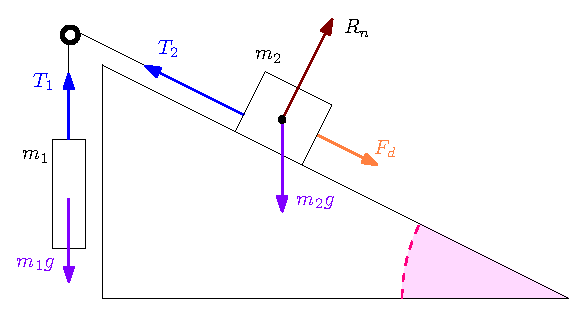
\includegraphics[width=0.7\textwidth ]{images/carrucola.eps}
    }
    \caption{Schema delle forze}
    \label{fig:carrucola}
\end{figure}
Si ipotizzi che il corpo di massa $m_1$ cada verso il basso, spostando il corpo di massa $m_2$ verso sinistra.
Per il primo corpo, si considera un sistema di riferimento in cui l'asse delle ordinate è parallelo alla 
direzione della gravità, per il secondo corpo si considera un sistema di riferimento in cui 
l'asse delle ascisse forma un angolo $\alpha$ con la linea dell'orizzone. \acc 
Analizziamo il moto del primo corpo, la sua forza avrà componente nulla sull'asse 
delle ascisse, sull'asse delle ordinate sarà 
$$ T_1-m_1g=m_1a_1$$
Il secondo corpo, si sposterà solamente lungo il piano, la sua forza avrà componente nulla sull'asse 
delle ordinate. 
$$\begin{cases}
    T_2-F_d+m_2g\sin\alpha=m_2a_2 \\ 
    R_n-m_2g\cos\alpha = 0
\end{cases}$$
Si ricordi che $F_d=\mu_dR_n$
$$\begin{cases}
    T_2-\mu_dR_n+m_2g\sin\alpha=m_2a_2 \\ 
    R_n-m_2g\cos\alpha = 0
\end{cases}$$
A tal punto si considerano due ulteriori ipotesi\begin{itemize}
    \item La massa del filo è trascurabile, quindi $T_1=T_2=T$ 
    \item Il filo è inesensibile, quindi $a_1=a_2=a$
\end{itemize}
Allora si può riscrivere il sistema per trovare $a$ 
$$\begin{cases}
    T-m_1g=m_1a \\
    T-\mu_dR_n+m_2g\sin\alpha=m_2a \\ 
    R_n-m_2g\cos\alpha = 0
\end{cases}$$$$\begin{cases}
    T=m_1(g+a) \\
    T-\mu_d(m_2g\cos\alpha )+m_2g\sin\alpha=m_2a \\ 
    R_n=m_2g\cos\alpha 
\end{cases}$$ 
A questo punto si risolve per $a$
$$ -m_1(g+a)-\mu_d(m_2g\cos\alpha )+m_2g\sin\alpha=m_2a$$
$$ a=\frac{m_2g\sin\alpha-\mu_dm_2g\cos\alpha-m_1g}{m_1+m_2}$$
è l'accelerazione del corpo 1 sull'asse verticale e del corpo 2 sul piano.
\subsubsection{Momento di un Sistema di Punti}
Come si è considerata la forza totale di un sistema è possibile considerare il momento. Si consideri un insieme di punti con diverse velocità, ed un'unico polo.\begin{center}
    \includegraphics[width=0.4\textwidth ]{images/momentoPunti.eps}
\end{center}
Sia $v_0$ la velocità del polo, il sistema dei momenti è $$ \begin{cases}
    M_1=\dfrac{db_1}{dt}+v_0\times r_1\\ 
    M_2=\dfrac{db_2}{dt}+v_0\times r_2\\
    \dots \\ 
    M_n=\dfrac{db_n}{dt}+v_0\times r_n
\end{cases}$$
Essendo che le forze interne si annullano, anche i momenti interni si annullano. Si consideri la somma dei momenti $$ (\dfrac{d}{dt}\sum{b_i})+v_0\times (\sum r_i)$$
si può riscrivere 
 $$ \dfrac{d}{dt}(\sum{r_i\times m_iv_i})+v_0\times (\sum r_i)$$
Sebbene la somma delle quantità di moto sia la quantità di moto del centro di massa di un sistema, la somma dei momenti \underline{non è} il momento del centro di massa.
\subsection{Sistemi Continui}
Quando un punto di massa $m$ rotea su una  circonferenza di raggio $r$ con una velocità angolare $\omega$ 
sappiamo idenitficare momento, quantità di moto del momento e momento di inerzia 
$$ \bar M = I\dot{\omega} \ \ \bar b = I\omega \ \ I=rm^2$$
Cosa si può dire dei corpi continui? Si vuole trovare il momento di inerzia di un bastone di legno di lunghezza $l$ che rotea attorno un certo asse.
\begin{center}
    \includegraphics[width=0.4\textwidth ]{images/bastone.pdf}
\end{center}
Sia $M$ la massa totale del bastone, non sappiamo come calcolare il momento di inerzia $I$ del bastone intero, ma è possibile considerare un tratto infinitesimo del bastone approssimabile ad un punto materiale, sia $x$ la 
distanza dal centro dell'asse al tratto infinitesimo, il momento di inerzia elementare sarà quindi.
$$ dI=x^2dM$$
Allora 
$$ I=\int dI=\int x^2dM$$
È necessario trovare una grandezza che metta in relazione la massa con la distanza del punto dall'asse (lunghezza), si definisce quindi la \textbf{densità}
$$ \frac{dM}{dl}=\lambda$$
Quindi 
$$I=\int_0^lx^2\lambda dx $$
Si considera la densità un valore costante, tale che la massa 
$$ M=\int_0^l\lambda dx = \lambda l$$
È possibile calcolare il momento di inerzia 
$$I=\int_0^lx^2\lambda dx =\lambda=\int_0^lx^2 dx =\lambda\frac{l^3}{3}$$
Si può esprimere in funzione della massa 
$$ I=\frac{1}{3}Ml^2$$
Si consideri il seguente esempio in cui l'asse di rotazione viene posto al centro del bastone.\begin{center}
    \includegraphics[width=0.5\textwidth ]{images/bastone2.pdf}
\end{center}
In questo caso cambiano gli estremi di integrazione 
$$ I=\int_{-\nicefrac{l}{2}}^{\nicefrac{l}{2}}x^2\lambda dx=\frac{1}{3}\lambda x^3\Bigg|_{-\nicefrac{l}{2}}^{\nicefrac{l}{2}}=\frac{1}{3}\lambda [\frac{l^3}{8}-(-\frac{l^3}{8})]= 
\frac{1}{12}Ml^2$$
\subsection{Rotazione di un Corpo Rigido}
Definiamo il cosiddetto \textit{pendolo composto}, si consideri corpo continuo arbitrario (verrà rappresentato 
come una lamina di ferro), tale corpo, ha un centro di massa $cm$. Si "infilza" il corpo con un asso in un 
certo punto.\begin{center}
    \includegraphics[width=0.5\textwidth ]{images/pendoloComposto.eps}
\end{center}
Sia $d$ la distanza dal punto di infilzamento ed il centro di massa, e sia $\theta$ l'angolo compreso fra il vettore gravità ed il vettore che va dal punto di infilzamento ed il centro di massa (di lunghezza $d$). Il corpo comincierà a ruotare attorno il punto di infilzamento, se ne vuole calcolare il momento. 
Sia $I_0$ il momento di inerzia del punto di infilzamento con polo nel centro di massa, l'equazione del moto 
è 
$$-mgd\sin\theta=-I_0\dfrac{d^2\theta}{dt^2}$$
Si approssima per $\theta$ piccoli dove $\sin\theta\simeq \theta$
$$ -mgd\theta=-I_0\dfrac{d^2\theta}{dt^2}$$
$$\dfrac{d^2\theta}{dt^2}+\frac{Mgd}{I_0}=0$$
È l'equazione del moto armonico, troviamo velocità angolare e periodo 
$$\omega = \sqrt{\frac{Mgd}{I_0}}  \ \ \ \ \ T=2\pi\sqrt{\frac{I_0}{Mgd}}$$
Come varia il periodo $T$ al variare di $d$? Apparentemente, potrebbe sembrare che che $T$ si comporti come 
$$ T(d)\propto \frac{1}{\sqrt{d}}$$
ma ciò è errato, in quanto va considerato il momento di inerzia che dipende proprio da $d$, infatti 
$$ I_0=I_{cm}+md^2$$
Dove $I_{cm}$ è il momento di inerzia del centro di massa, ed è costante. Si ha quindi 
$$ T(d)=2\pi\sqrt{\frac{I_{cm}+md^2}{mgd}}$$
Quindi, se infilzassimo il corpo esattamente nel centro di massa, $d=0\implies T=\infty \implies$ non ci sarebbero oscillazioni. Più il corpo viene infilzato lontano dal suo centro di massa, più le oscillazioni 
saranno frequenti.\begin{center}
    \begin{tikzpicture}[scale=1, transform shape]
		\begin{axis}[
		ymin=4,
		ymax = 10,
		xmin=0.3,
		xmax = 6,
		axis lines = left,
		xtick distance=1, ytick distance=1,
		grid style=dashed,
		ymajorgrids=true,
		xmajorgrids=true,
		xlabel = \(d\),
		ylabel = {\(T(d)\)},
		]
		%Below the red parabola is defined
		\addplot [
		domain=0:6,
		samples=20,
		color=blue,
		]
		{2*pi*sqrt((5+x^2)/(9.81*x))};
		\end{axis}
		\end{tikzpicture}
\end{center}
\flowerLine
\section{Rotolamento}
In questa sezione verrà definito il rotolamento di una ruota. Si consideri appunto, una ruota di una auto che si muove, in ogni istante, un punto materiale che si trova sulla frontiera della ruota ha una velocità che è 
composizione di 2 velocità : La velocità di traslazione (del centro di massa) $v_c$ e la velocità tangenziale $\omega r$ di rotazione attorno al centro.
\begin{center}
    \includegraphics[width=0.5\textwidth ]{images/rotolamento.pdf}
\end{center}
La velocità totale del punto è $v=v_c+\omega r$, nel preciso punto di contatto della ruota con il suolo, la velocità angolare sarà di eguale direzione ma verso opposto della velocità di traslazione. La condizione di 
\textbf{purto rotoalmento} si ha quando $|\omega r |= |v_c|$. \acc 
Si consideri adesso una ruota di raggio $R$ e massa $M$ sollevata dal suolo, a cui viene data una velocità angolare $\omega$. Abbassando pian piano la ruota, arriverà un istante in cui tocca il suolo, in quell'istante preciso, 
l'\textit{attrito dinamico} costituisce una forza esterna.
$$ F_dR=I\dot{\omega}$$
Si vuole descrivere il moto del centro di massa, sia $x_{cm}$ la sua posizione 
$$ \begin{cases}
    x_{cm}(t)=\frac{1}{2}a_{cm}t^2+\frac{1}{2}\frac{F_d}{M}t^2 \\ 
    v_{cm}=a_{cm}t=\frac{F_d}{M}t
\end{cases}$$
La velocità angolare invece andrà diminuendo, sia $\omega_0$ la velocità angolare iniziale 
$$ \omega = -\omega_0+\dot{\omega}t+\frac{F_dR}{I}t$$
Lo strusciamento fa diminuire la velocità angolare.
\begin{center}
    \includegraphics[width=0.7\textwidth ]{images/puroRot.eps}
\end{center}
\subsubsection{Rotolamento su un Piano Inclinato}
Si consideri un generico corpo su un piano inclinato posto ad un altezza $h$, essendo che l'energia cinetica si conserva, la sua energia cinetica iniziale è identica a quella finale 
$$ \frac{1}{2}mv^2=mgh$$
La velocità del corpo una volta finita la corsa sul piano sarà $$ v=\sqrt{2gh}$$
Supponiamo ora che sul piano ci sia un disco che rotola. L'energia cinetica è 
$$ \frac{1}{2}mv_c^2+\frac{1}{2}I\omega ^2$$
Essa si conserva quindi 
$$ \frac{1}{2}mv_c^2+\frac{1}{2}I\omega ^2=mgh$$
L'energia potenziale si "suddividerà" fra la componente traslatoria e la componente rotatoria, per un disco, 
$I=\frac{1}{2}mR^2$, la velocità di traslazione a fine corsa sarà 
$$ v_c=\sqrt{mgh\frac{1}{m+\nicefrac{I}{R^2}}}=\sqrt{\frac{2mgh}{m+\nicefrac{1}{2}m}}=\sqrt{\nicefrac{2}{3}}\sqrt{2gh}$$
Quindi la velocità del corpo che ruota sarà minore della velocità del corpo che striscia, dato che l'energia di traslazione mancante a tale corpo sarà contenuta nella velocità di rotazione acquisita.\flowerLine 
\section{Sistemi Equivalenti di Forze}
Date due forze applicate ad un sistema, si vuole trovare una forza unica risultante che sia equivalente alle due (se sostituita alle forze originali, la dinamica del sistema rimane invariata). Verranno analizzati 3 casi. 
\subsubsection{Caso 1}
Si considerano due forze parallele $F_1$ ed $F_2$ applicate in due punti distinti distanti $d$.\begin{center}
    \includegraphics[width=0.3\textwidth ]{images/forzeEq1.eps}
\end{center}
Definisco sull'asse che congiunge i due punti due forze uguali e contrarie (di intensità arbitraria) $f_1,f_2$, 
considerando poi altra due forze risultanti $R_1=F_1+f_1$ ed $R_2=F_2+f_2$.
\begin{center}
    \includegraphics[width=0.4\textwidth ]{images/forzeEq2.eps}
\end{center}
Si considera il punto $O$ come incontro dei prolungamenti di $R_1$ e $R_2$, in cui si applica $R_1+R_2$, il cui incontro con l'asse congiungente i dui punti originali sarà chiamato $C$ e sarà il punto in cui, dovrà essere applicata la forza $F_1+F_2$ per rendere il sistema equivalente..
\begin{center}
    \includegraphics[width=0.4\textwidth ]{images/forzeEq3.eps}
\end{center}
In ogni punto i momenti delle forze saranno equivalenti 
$$ \bar M_F=\bar M_{F_1}+\bar M_{F_2}$$
Il momento applicato nel punto $C$ sarà nullo quindi 
$$ 0=F_1d_1-F_2d_2\implies \frac{d_1}{d_2}=\frac{F_2}{F_1}$$
Trovando $d_1,d_2$ si definisce il preciso punto di applicazione della forza equivalente.
\subsubsection{Caso 2}
Si considerano adesso due forze parellele ma in verso opposto, applicate nei punti $P_1$ e $P_2$, aventi intensità diverse. La forza risultante avrà intensità pari alla differenza fra le due forze, e sarà diretta nel verso della forza con intensità maggiore.\acc 
Il punto di applicazione $C$, si troverà sulla retta che congiunge $P_1$ e $P_2$, in una 
posizione determinata dalal relazione $$ -F_1d_1+F_2d_2=0\implies \frac{d_1}{d_2}=\frac{F_2}{F_1}$$
\begin{center}
    \includegraphics[width=0.5\textwidth ]{images/forzeEq4.eps}
\end{center}
\subsubsection{Caso 3 : Coppia}
Si considerino due forze parallelle dirette in verso opposto e di uguale intensita $F_1=-F_2$. In questo specifico caso, non è possibile riprodurre l'effetto delle due forze con una singola forza.\begin{center}
    \includegraphics[width=0.3\textwidth ]{images/coppia.eps}
\end{center}
In questo specifico caso, la somma dei momenti delle due forze è \textit{invariante rispetto il punto di applicazione}, sia $O$ un generico punto 
\begin{eqnarray}
    M=M_1+M_2=OP_1\times F_1 + OP_2\times F_2=OP_1\times F_1 + OP_2\times (-F_1)=\\ 
    F_1(OP_1-OP_2)=P_2P_1\times F_1
\end{eqnarray} 
Il momento della coppia di forze è normale al piano delle due forze, sia $b$ la distanza fra $P_1$ e $P_2$, l'intensità della forza è $|F_1|b=|F_2|b$. La coppia è un sistema di forze \textbf{irriducibile} ed è completamente individuata dal suo momento.\begin{quote}
   Un  momento di forze può essere rappresentato per mezzo di una qualsiasi coppia di forze che ha quel momento.
\end{quote}
\chapter{Forza Elettrica}
Gli atomi sono i costituenti della materia, sono formati da un nucleo (protoni e neutroni) e da elettroni che si trovano attorno ad esso. In passato sono stati osservati fenomeni di forza elettrica senza però conoscerne le cause. Ad esempio, strofinando una bacchetta di vetro su un maglione di lana si potrà osservare che questa acquisirà la proprietà di attirare a se (esercitare una forza) su oggetti leggeri (come un pezzo di carta).\acc 
La \textbf{carica} è una proprietà fondamentale della materia, si misura in \textit{Coloumb} $C$ , ed è quantizzata, in particolare, la carica elementare è quella posseduta da un protone o da un elettrone, questi ultimi infatti hanno carica di eguale modulo, ma segno opposto.\begin{center}
    \begin{tabular}{|l|l|}
        \hline
        Particella & Carica ($C$)                \\ \hline
        elettrone  & $-1.602177335\cdot10^{-19}$ \\ \hline
        protone    & $+1.602177335\cdot10^{-19}$ \\ \hline
        neutrone   & 0                           \\ \hline
        \end{tabular}
\end{center}
Essendo che in un atomo il numero dei protoni coincide con il numero degli elettroni, questo risulta elettricamente neutro, quando si strofina la bacchetta di vetro sulla lana, questa riesce a "strappare" degli elettroni, e caricarsi negativamente, acquisendo una carica non neutra.\acc 
La \textbf{Forza Elettrica} è una forza che agisce sui corpo carichi, in particolare, un corpo carico negativamente eserciterà una forza attrattiva sui corpi carichi positivamente, e repulsiva sui corpi carichi negativamente. Analogo ma contrario con i corpi carichi positivamente.\begin{center}
    \includegraphics[width=1\textwidth ]{images/cariche.pdf}
\end{center}
Si considerino due corpi carichi, di carica $q$ e $q_0$, sia $\hat r$ il versore congiungente il primo corpo con il secondo, e sia $r$ la loro distanza. Il corpo di carica $q$ eserciterà sul corpo di carica $q_0$ una forza 
$$ \bar F = \frac{1}{4\pi\varepsilon_0}\frac{q\cdot q_0}{r^2}\hat r$$
Il termine $\varepsilon_0$ è detta \textbf{costante dielettrica nel vuoto} e vale 
$$ \varepsilon_0=8.8542\cdot10^{-12}\frac{C^2}{Nm^2}$$
\textbf{Esempio} : L'elettrone ed il protone di un atomo di idrogeno si trovano ad una distanza media di 
$$ r=0.53\cdot10^{-10}m$$
La forza applicata sulle particelle ha modulo 
$$ \frac{1}{4\pi8.8542\cdot10^{-12}}\frac{-(1.602177335\cdot10^{-19})^2}{(0.53\cdot10^{-10})^2}=8.20\cdot 10^{-8}N$$
\end{document}